% !TeX program = pdflatex
% !TeX root=./main.tex
% Edit by:XAjzh and sikouhjw

\chapter{多维随机变量及其分布}\label{cha:3}
在有些随机现象中, 对每个样本点 $\omega$ 只用一个随机变量去描述是不够的, 
譬如要研究儿童的生长发育情况, 仅研究儿童的身高 $X(\omega)$ 或仅研究其体重 $Y(\omega)$都是片面的, 
有必要把 $X(\omega)$ 和 $Y(\omega)$ 作为一个整体来考虑, 讨论它们总体变化的统计规律性, 
进一步可以讨论 $X(\omega)$ 与 $Y(\omega)$ 之间的关系, 在有些随机现象中, 甚至要同时研究二个以上随机变量. 

如何来研究多维随机变量的统计规律性呢, 仿一维随机变量, 我们先研究联合分布函数, 
然后研究离散随机变量的联合分布列、连续随机变量的联合密度函数. 

\section{多维随机变量及其联合分布}\label{sec:3.1}

\subsection{多维随机变量}\label{ssec:3.1.1}
下面我们先给出 $n$ 维随机变量的定义. 
\begin{definition}{随机变量}{3.1.1}
	如果 $X_1(\omega),X_2(\omega),\ldots,X_n(\omega)$ 是定义在同一
	样本空间 $\Omega=\left\{\omega\right\}$ 上的 $n$ 个随机变量, 则称
	\[
	X(\omega)=(X_1(\omega),X_2(\omega),\ldots,X_n(\omega))
	\]
	为 $n$ 维(或 $n$ 元)\textbf{随机变量}\index{S!随机变量}或\textbf{随机向量}\index{S!随机向量}. 
\end{definition}
注意, 多维随机变量的关键是定义在同一样本空间上, 对于不同样本空间上的两个随机变量, 我们只能在
乘积空间 $\Omega_1\times \Omega_2=\left\{(\omega_1,\omega_2);\omega_1 \in \Omega_1,\omega_2 \in \Omega_2 \right\}$ 上讨论, 
 这要用到更多的工具, 本章将不涉及这类问题. 
      
 在实际问题中, 多维随机变量的情况是经常会遇到的譬如
  \begin{itemize}
  	\item 在研究四岁至六岁儿童的生长发育情况时, 我们感兴趣于每个儿童 (样本点 $\omega$) 的身高 $X_1(\omega)$ 
  	和体重 $X_2(\omega)$ . 这里 $(X_1(\omega),X_2(\omega))$ 是一个二维随机变量. 
  	\item 在研究每个家庭的支出情况时, 我们感兴趣于每个家庭 (样本点 $\omega$) 的衣食住行四个方面, 
  	若用 $X_1(\omega),X_2(\omega),X_3(\omega),X_4(\omega)$ 分别表示衣食住行的花费占其家庭总收人的百分比, 
  	则 $(X_1(\omega),X_2(\omega),X_3(\omega),X_4(\omega))$ 就是一个四维随机变量. 
  \end{itemize}

  \subsection{联合分布函数}\label{ssec:3.1.2}
  \begin{definition}{联合分布函数}{3.1.2}
  	对任意的 $n$ 个实数 $x_1,x_2,\ldots,x_n ,$ 则 $n$ 个事件 $\{X_1\leq x_1\},\{X_2 \leq x_2\},\ldots,\{X_n\leq x_n\}$ 同时发生的概率
    \begin{equation}
    	F\left(x_{1}, x_{2}, \cdots, x_{n}\right)=P\left(X_{1} \leq x_{1}, X_{2} \leq x_{2}, \ldots, X_{n} \leq x_{n}\right)\label{eq:3.1.1}
    \end{equation}
	称为 $n$ 维随机变量 $(X_1,X_2,\ldots,X_n)$ 的\textbf{联合分布函数}\index{L!联合分布函数}. 
  \end{definition}
   本章主要研究二维随机变量, 二维以上的情况可类似进行. 

   在二维随机变量 $(X,Y)$ 场合, 联合分布函数 $F(x,y)=P(X\leq x,Y\leq y)$ 是事件 $\{X\leq x\}$ 与 $\{Y \leq y\}$ 同时发生(交)的概率. 
   如果将二维随机变量 $(X,Y)$ 看成是平面上随机点的坐标, 那么联合分布函数 $F(x,y)$ 在 $(x,y)$ 处的函数值就是随机点 $(X, Y)$ 落在
   以 $(x,y)$ 为右上角的无穷矩形内的概率, 见图~\ref{fig:3.1.1} .
   \begin{figure}[htbp]
   	\centering
   	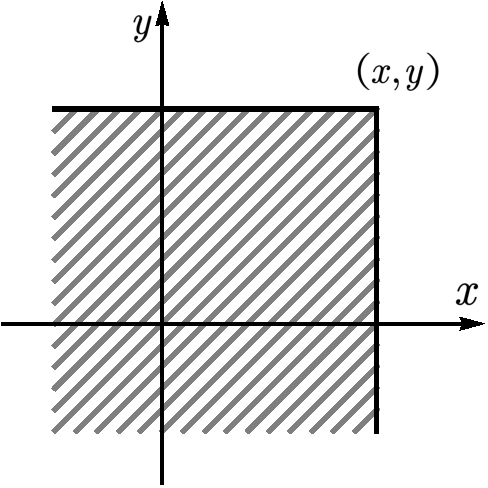
\includegraphics[width=0.4\textwidth]{fig3-1-1.pdf}
   	\caption{联合分布函数示意图}\label{fig:3.1.1}
   \end{figure}
   \begin{theorem}{}{3.1.1}
   	任一二维联合分布函数 $F(x,y)$ 必具有如下四条基本性质: 
    \begin{enumerate}
    	\item \textbf{单调性}\quad $F(x,y)$ 分别对 $x$ 或 $y$ 是单调不减的,即
    	\begin{itemize}
    		\item 当 $x_1<x_2$ 时, 有 $F(x_1,y)\leq F(x_2,y)$.
    		\item 当 $y_1<y_2$ 时, 有 $F(x,y_1)\leq F(x,y_2)$. 
    	\end{itemize}
    	\item \textbf{有界性}\quad 对任意的 $x$ 和 $y$, 有 $0\leq F(x,y) \leq 1$, 且
    	\begin{align*}
    		&F(-\infty,y)=\lim_{x\to -\infty}F(x,y)=0,	&\hspace*{3cm} \\
    		&F(x,-\infty)=\lim_{y\to -\infty}F(x,y)=0,	&\\
    		&F(+\infty,+\infty)=\lim_{x,y\to +\infty}(x,y)=1.&
    	\end{align*}
    	\item \textbf{右连续性}\quad  对每个变量都是右连续的,即
    		\begin{align*} 
    			F(x+0, y) &=F(x, y), &\hspace*{3cm} \\ 
    			F(x, y+0) &=F(x, y). &
    		\end{align*}
    	\item \textbf{非负性}\quad 对任意的 $a<b,c<d$ 有
    		\begin{equation*}
    		 	P(a<X \leq b, c<Y \leq d)= F(b, d)-F(a, d)-F(b, c)+ F(a, c) \geq 0 .
    		\end{equation*}
    \end{enumerate}
   \end{theorem}
   \begin{proof}
    	\begin{enumerate}
    		\item  因为当 $x_1<x_2$ 时, 有 $\{X_1\leq x_1\} \subset \{X_2 \leq x_2\}$, 所以对任意给定的 $y$ 有
    		\[
    			\left\{X \leq x_{1}, Y \leq y\right\} \subseteq \{ X \leq x_{2}, Y \leq y \},
    		\]
    		由此可得
    		\[
    			F\left(x_{1}, y\right)=P\left(X \leq x_{1}, Y \leq y\right) \leq 
    			P\left(X \leq x_{2}, Y \leq y\right)=F\left(x_{2}, y\right),
    		\]
    		即 $F(x,y)$ 关于 $x$ 是单调不减的, 同理可证 $F(x,y)$ 关于 $y$ 是单调不减的.
    		\item 由概率的性质可知 $0\leq F(x,y) \leq 1$. 又因为对任意的正整数 $n$ 有
    		\begin{align*}
    			&\lim_{x\to -\infty}\{X\leq x\}=\lim_{n\to +\infty}\bigcap_{m=1}^n \{X\leq -m\}=\varnothing,	\\
    			&\lim_{x\to +\infty}\{X\leq x\}=\lim_{n\to +\infty}\bigcup_{m=1}^n\{X\leq m\}=\Omega,
    		\end{align*}
    		对 $Y \leq y$ 也类似可得. 再由概率的连续性, 就可得
    		\[
    		 	F(-\infty, y)=F(x,-\infty)=0; \quad F(+\infty,+\infty)=1.
    		\]
    		\item 固定 $y$, 仿一维分布函数右连续的证明, 就可得知 $F(x, y)$ 关于 $x$ 是右连续的. 同样固定 $x$ 可
    		证得 $F(x,y)$ 关于 $y$ 是右连续的.
        	\item 只需证
        	\[
        	 	P(a<X \leq b, c<Y \leq d)=F(b, d)-F(a, d)-F(b, c)+F(a, c).
        	\]
        	为此记 ( 见图~\ref{fig:3.1.2} )
        	\[
        	 	A=\{X \leqslant a\}, \quad B=\{ X \leqslant b \}, \quad C=\{Y \leqslant c\}, \quad D=\{Y \leqslant d\},
        	\]
        	考虑到
        	\[
        	 	\{ a<X \leqslant b \}=B-A=B \cap \overline{A}, \quad\{c<Y \leqslant d\}=D-C=D \cap \overline{C},
        	\]
        	且 $A \subset B, C\subset D,$ 由此可得
        	\begin{align*}
        		 0 & \leqslant P(a<X \leqslant b, c<Y \leqslant d) \\ 
        		 &=P(B \cap \overline{A} \cap D \cap \overline{C}) \\ 
        		 &=P(B D-(A \cup C)) \\ 
        		 &=P(B D)-P(A B D \cup B C D) \\ 
        		 &=P(B D)-P(A D \cup B C) \\ 
        		 &=P(B D)-P(A D)-P(B C)+P(A B C D) \\ 
        		 &=P(B D)-P(A D)-P(B C)+P(A C ) \\ 
        		 &=P(B D)-P(A D)-P(B C)+P(A B C D) \\ 
        		 &=F(b, d)-F(a, d)-F(b, c)+F(a, c). 
        	\end{align*}
    	\end{enumerate}
    \end{proof}
   \begin{figure}[htbp]
   	\centering
   	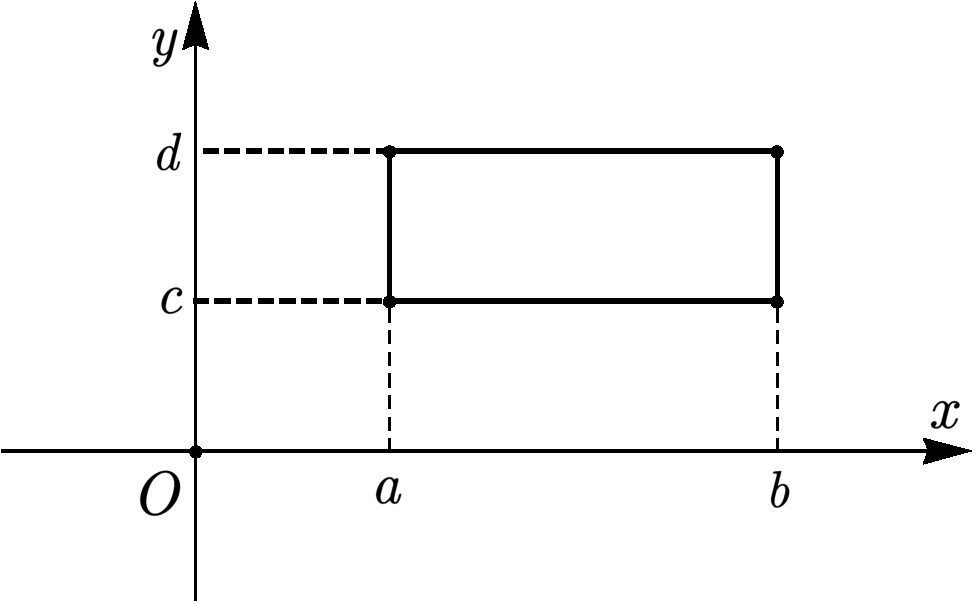
\includegraphics[width=0.4\textwidth]{fig3-1-2.pdf}
   	\caption{二维随机变量 $(X,Y)$ 落在矩形中的情况}\label{fig:3.1.2}
   \end{figure}
   还可证明,具有上述四条性质的二元函数 $F(x,y)$ 一定是某个二维随机变量的分布函数.

   任一二维分布函数 $F(x,y)$ 必具有上述四条性质, 其中性质 \textit{4} 是二维场合特有的, 也是合理的. 但性质 \textit{4} 不能
   由前三条性质推出, 必须单独列出, 且仅满足前三条性质是不够的, 因为存在这样的二元函数 $G(x,y)$ 满足
   以上性质 \textit{1,2,3}, 但它不满足性质 \textit{4}, 见下面例子.

   \begin{example}\label{exam:3.1.1}
   	二元函数
   	\[
   	 	G(x,y)=\begin{cases}
   	 		0,	& x+y<0;\\
   	 		1,	& x+y\geq 0 \\
   	 	\end{cases}
   	\]
   	满足二维分布函数的性质 \textit{1,2,3}, 但它不满足性质 \textit{4}.

    这从 $G(x,y)$ 的定义可看出: 若用 $x+y=0$ 将平面 $xOy$ 一分为二, 则
 
    $G(x,y)$ 在右上半平面 $(x+y\geq 0)$ 取值为1,
   
    $G(x,y)$ 在左下半平面 $(x+y\geq 0)$ 取值为0,

    $G(x,y)$ 具有非降性、有界性和右连续性, 但在正方形区域 $\{(x,y); -1\leq x\leq 1,-1\leq y\leq 1\}$的四个顶点上, 右上
    三个顶点位于右上半闭平面, 只有左下顶点 $(-1,-1)$ 位于左下半开平面, 故有
    \[
     	G(1,1)-G(1,-1)-G(-1,1)+G(-1,-1)=1-1-1+0=-1<0,
    \]
	所以 $G(x,y)$ 不满足性质 \textit{4}, 故 $G(x,y)$ 不能成为某二维随机变量的分布函数.
   \end{example}

   \subsection{联合分布列}\label{ssec:3.1.3}

   \begin{definition}{联合分布列}{3.1.3}
		如果二维随机变量 $(X,Y)$ 只取有限个或可列个数对 $(x_i,y_j)$, 则称 $(X,Y)$ 为二维离散随机变量, 称
    \begin{equation}\label{eq:3.1.2}
     	p_{i j}=P\left(X=x_{i}, Y=y_{j}\right), \quad i, j=1,2, \ldots
    \end{equation}
   	为 $(X,Y)$ 的\textbf{联合分布列}\index{L!联合分布列}, 也可如下用表格形式记联合分布列.
   \end{definition}
   \begin{center}
   		\begin{tabularx}{0.8\textwidth}{ZZZZZZ}
   		\toprule
   		 & \multicolumn{5}{c}{$Y$} \\
   		 \cmidrule{2-6} 
   		 $X$	&	$y_1$&	$y_2$&	\ldots&	$y_j$& \ldots	\\
   		 \midrule 
   		 $x_1$& $p_{11}$ & $p_{12}$ & \ldots & $p_{1j}$ & \ldots \\
   		 \midrule 
   		 $x_2$& $p_{21}$ & $p_{22}$ & \ldots & $p_{2j}$ & \ldots \\
   		 \midrule 
   		 $\vdots$& $\vdots$ & $\vdots$ & $\ddots$ & $\vdots$ & $\ddots$ \\
   		 \midrule 
   		$x_i$ & $p_{i1}$ & $p_{i2}$ & \ldots & $p_{ij}$  & \ldots \\
   		\midrule 
   		 $\vdots$& $\vdots$ & $\vdots$ & $\ddots$ & $\vdots$ & $\ddots$ \\
   		 \bottomrule
   		\end{tabularx} 
   \end{center}
   联合分布函数的基本性质:
   \begin{enumerate}
   	\item 非负性: $p_{ij}\geq 0$;
   	\item 正则性: $\sum_{i=1}^{+\infty}\sum_{j=1}^{+\infty}p_{ij}=1$.
   \end{enumerate}
   求二维离散随机变量的联合分布列, 关键是写出二维随机变量的可能取的数对及其发生的概率.

   \begin{example}\label{exam:3.1.2}
   		从 1,2,3,4 中任取一数记为 $X$, 再从 $1,\ldots,X$ 中任取一数记为 $Y$. 求 $(X,Y)$ 的联合分布列及 $P(X=Y)$.     
   \end{example}
   \begin{solution}
   		$(X,Y)$ 为二维离散随机变量, 其中 $X$ 的分布列为
         \[  
         	 P(X=i)=1/4,i=1,2,3,4.
         \]
		$Y$ 的可能取值也是 $1,2,3,4$, 若记 $j$ 为 $Y$ 的取值,

		 则当 $j>i$ 时,有 $P(X=i,Y=j)=P(B)=0$.
  
  		当 $1\leq j \leq i \leq 4$ 时,由乘法公式
  		\[
  		 	P(X=i, Y=j)=P(X=i) P(Y=j | X=i)=\frac{1}{4} \times \frac{1}{i}.
  		\]
		所以得 $(X,Y)$ 的联合分布列为
		\begin{center}
			\begin{tabularx}{0.8\textwidth}{ZZZZZ}
			\toprule
			 & \multicolumn{4}{c}{$Y$} 		 \\ 
			 \cmidrule{2-5}
			 $X$&  	1	&  2	&  3&  		4\\ 
			 \midrule
			 1 	&  1/4	&  0	&  0&  		0\\
			 \midrule
			 2	&  1/8	& 1/8 	&  0&  		0\\ 
			 \midrule
			 3	& 1/12	&  1/12	&  1/12&	0\\ 
			 \midrule
			 4&  1/16	&  1/16	&  1/16&  1/16\\ 
			 \bottomrule
			\end{tabularx} 
		\end{center}
		由此可算得事件 $\{X=Y\}$ 的概率为
		\[
		 	P(X=Y)=p_{11}+p_{22}+p_{33}+p_{44}=\frac{1}{4}+\frac{1}{8}+\frac{1}{12}+\frac{1}{12}=\frac{25}{48}=0.5208
		\]
   \end{solution}
   \subsection{联合密度函数}\label{ssec:3.1.4}
   \begin{definition}{联合密度函数}{3.1.4}
   	如果存在二元非负函数 $p(x,y)$, 使得二维随机变量 $(X,Y)$ 的分布函数 $F(x,y)$ 可表示为
   	\begin{equation}\label{eq:3.1.3}
   	 	F(x, y)=\int_{-\infty}^{x} \int_{-\infty}^{y} p(u, v) \dd v \dd u
   	\end{equation}
   	则称 $(X,Y)$ 为二维连续随机变量, 称 $p(u,v)$ 为 $(X,Y)$ 的\textbf{联合密度函数}\index{L!联合密度函数}.
   \end{definition}
   在 $F(x,y)$ 偏导数存在的点上有
   \[
    	p(x, y)=\frac{\partial^{2}}{\partial x \partial y} F(x, y).
   \]
   \textbf{联合密度函数的基本性质}:
   \begin{enumerate}
   	\item \textbf{非负性}: $p(u,v)\geq 0$ 
   	\item \textbf{正则性}: $\int_{-\infty}^{+\infty} \int_{-\infty}^{+\infty} p(u, v) \dd v \dd u=1$
   \end{enumerate}
   给出联合密度函数 $p(x,y)$, 就可以求有关事件的概率了. 若 $G$ 为平面上的一个区域, 
   则事件 $\{(X,Y) \in G\}$ 的概率可表示为在 $G$ 上对 $p(x,y)$的二重积分:
   \begin{equation}\label{eq:3.1.4}
    	P((X, Y) \in G)=\iint_{G} p(x, y) \dd x \dd y.
   \end{equation}
   在具体使用上式时, 要注意积分范围是 $p(x,y)$ 的非零区域与 $G$ 的交集部分, 然后设法化成累次积分, 最后计算出结果.
   \begin{example}\label{exam:3.1.3}
   		设 $(X,Y)$ 联合密度函数为
   		\[
   		p(x, y)=\left\{
   		\begin{array}{cc}
   		6 \ee^{-2 x-3 y}, & x>0, y>0; \\
   		0, & \text{其他} .
   		\end{array}\right.
   		\]
   		试求: $(1)\; P(X<1,Y>1); \; (2)\; P(X>Y)$.
   \end{example}
   \begin{solution}
  		\begin{enumerate}
  		\item 积分区域见图~\ref{fig:3.1.3a} 中的阴影部分, 
  		\begin{align*} 
  		 P(X<1, Y>1) &=\int_{1}^{+\infty} \int_{0}^{1} 6 \ee^{-2 x-3 y} \dd x \dd y \\
  		 &=6 \int_{0}^{1} \ee^{-2 x} \dd x \int_{1}^{+\infty} \ee^{-3 x} \dd y \\ 
  		 &=\left(1-\ee^{-2}\right) \ee^{-3}=0.0430. 
  		\end{align*}
  		\item 积分区域见图~\ref{fig:3.1.3b} 中的阴影部分, 从而容易写出累次积分.
  		\begin{align*} 
  		 P(X>Y) &=\int_{0}^{+\infty} \int_{0}^{x} 6 \ee^{-2 x} \ee^{-3 y} \dd y \dd x=
  		 \int_{0}^{+\infty} 2 \ee^{-2 x}\left(1-\ee^{-3 x}\right) \dd x \\ 
  		 &=\left[-\ee^{-2 x}+\frac{1}{5} \ee^{-5 x}\right]_{0}^{+\infty}=1-\frac{1}{5}=\frac{4}{5} .
  		\end{align*}
  		\end{enumerate}             
   \end{solution}
   \begin{figure}[htbp]
   \centering
   \subfloat[$\{x<1,y>1\}$ 区域 $D_1$]{\label{fig:3.1.3a}
   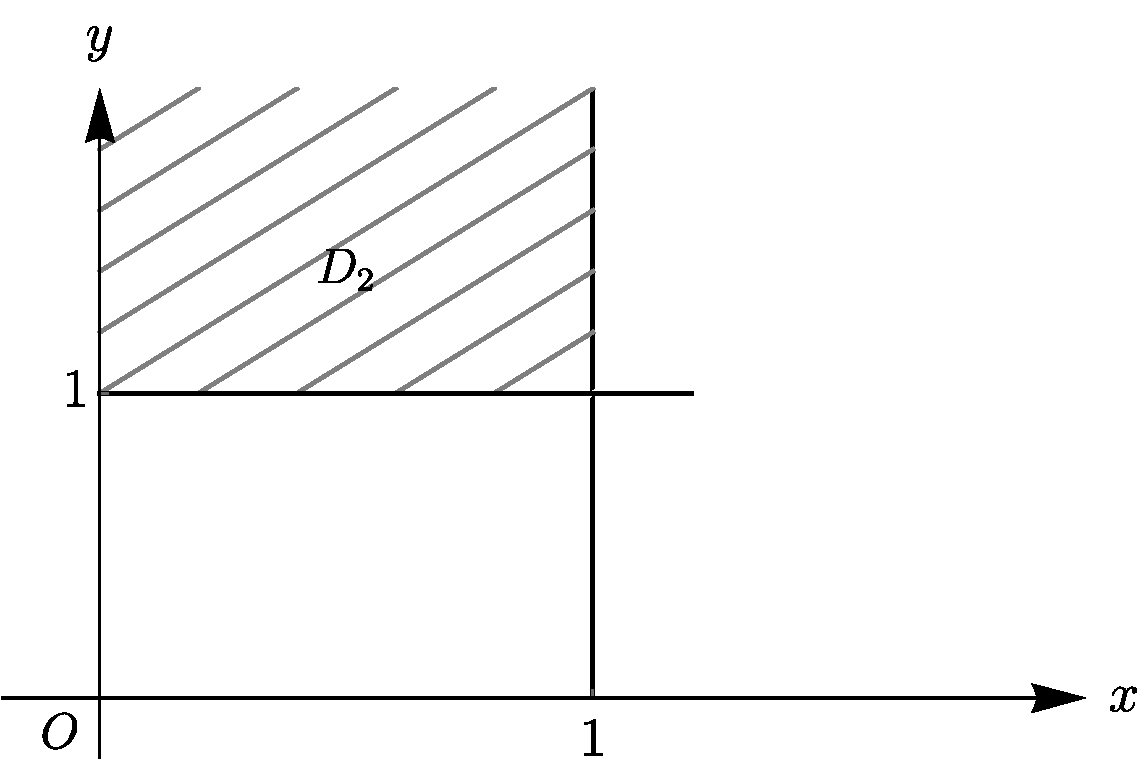
\includegraphics[width=0.4\textwidth]{fig3-1-3a.pdf}
   }\qquad
   \subfloat[$\{x>y\}$ 区域 $D_2$]{\label{fig:3.1.3b}
   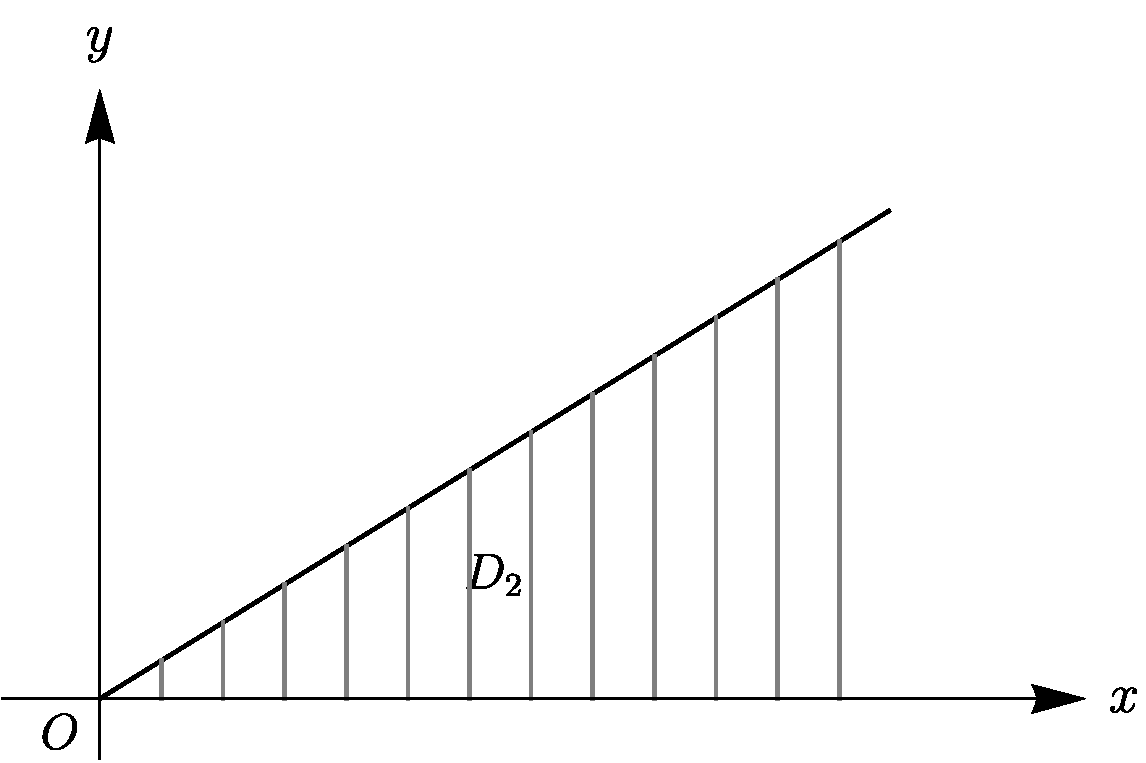
\includegraphics[width=0.4\textwidth]{fig3-1-3b.pdf}
   }
   \caption{$p(x,y)$ 的非零区域与有关事件的交集部分}\label{fig:3.1.3}
   \end{figure}
   
  \subsection{常用多维分布}\label{ssec:3.1.5}
  下面介绍一些多维随机变量的常用分布. 
   
  \textbf{一、多项分布 }
   
  多项分布是重要的多维离散分布, 它是二项分布的推广.
  
  进行 $n$ 次独立重复试验, 如果每次试验有 $r$ 个可能结果: $A_1, A_2$,\ldots,$A_r$, 且每次试验中 $A_i$ 发生的
  概率为 $p_{i}=P\left(A_{i}\right), i=1,2, \ldots, r . p_{1}+p_{2}+\cdots+p_{r}=1$.
  记 $X_i$ 为 $n$ 次独立重复试验中 $A_i$ 出现的次数, $i=1,2,\ldots,r$. 则 $(X_1,X_2,\ldots,X_r)$ 
  取值 $(n_1,n_2,\ldots,n_r)$ 的概率, 即 $A_1$ 出现 $n_1$ 次, $A_2$ 出现$n_2$ 次\ldots\ldots $A_r$ 出现 $n_r$ 次的概率为
  \begin{equation}
	  P\left(X_{1}=n_{1}, X_{2}=n_{2}, \ldots, X_{r}=n_{r}\right)=\frac{n !}{n_{1} ! n_{2} ! \cdots n_{r} !} p_{1}^{n_{1}} p_{2}^{n_{2}} \ldots p_{r}^{n_r},
  \end{equation}
  其中 $n=n_1+n_2+\cdots+n_r$.
  
  这个联合分布列称为 $r$ 项分布, 又称多项分布, 记为 $M(n,p_1,p_2,\ldots,p_r)$. 这个概率
  是多项式 $(p_1+p_2+\cdots+p_r)^n$ 展开式中的一项, 故其和为 1. 当 $r=2$ 时, 即为二项分布.
  \begin{example}\label{exam:3.1.4}
    一批产品共有 100 件, 其中一等品 60 件、二等品 30 件、三等品 10 件. 
    从这批产品中有放回地任取3件, 以 $X$ 和 $Y$ 分别表示取出的 3 件产品中一等品、二等品的件数, 求二维随机变量 $(X,Y)$ 的联合分布列.
  \end{example}
  \begin{solution}
    因为 $X$ 和 $Y$ 的可能取值都是 0,1,2,3, 所以记 $(X,Y)$ 的联合分布列为
    \begin{center}
      \begin{tabularx}{0.8\textwidth}{ZZZZZ}
        \toprule
          & \multicolumn{4}{c}{$Y$} \\
        \cmidrule{2-5}
        $X$ & 0&  1&  2&  3 \\
        \midrule
        0&  $p_{00}$& $p_{01}$& $p_{02}$& $p_{03}$\\
        \midrule
        1&  $p_{10}$& $p_{11}$& $p_{12}$& $p_{13}$\\
        \midrule
        2&  $p_{20}$& $p_{21}$& $p_{22}$& $p_{23}$\\
        \midrule
        3&  $p_{30}$& $p_{31}$& $p_{32}$& $p_{33}$\\
        \bottomrule
      \end{tabularx}
    \end{center}
    当 $i+j>3$ 时, 有 $p_{ij}=0$, 即
    \[
      p_{13}=p_{22}=p_{23}=p_{31}=p_{32}=p_{33}=0.
    \]
    而当 $i+j\leq 3$ 时, 事件 $\{X=i,Y=j\}$ 表示: 取出的 3 件产品中有 $i$ 件一等品、$j$ 件二等品、$3-i-j$ 件三等品的件数, 
    所以有放回地抽取时, 对 $i+j\leq 3$, 有
    \[
      p_{i j}=\frac{3 !}{i ! j !(3-i-j) !}\left(\frac{6}{10}\right)^{i}\left(\frac{3}{10}\right)^{j}\left(\frac{1}{10}\right)^{3-i-j}.
    \]
    由以上公式, 就可具体算出 $(X,Y)$ 的联合分布列为
    \begin{center}
      \begin{tabularx}{0.8\textwidth}{ZZZZZ}
        \toprule
          & \multicolumn{4}{c}{$Y$} \\
        \cmidrule{2-5}
        $X$ & 0&  1&  2&  3 \\
        \midrule
        0&  0.001   & 0.009   & 0.027   & 0.027   \\
        \midrule
        1&  0.018   & 0.108   & 0.162   & 0       \\
        \midrule
        2&  0.108   & 0.324   & 0       & 0       \\
        \midrule
        3&  0.216   & 0       & 0       & 0       \\
        \bottomrule
      \end{tabularx}
    \end{center}
  \end{solution}
  有此联合分布列, 就可计算有关事件的概率, 譬如
  \begin{align*}
    P(X \leq 1, Y \leq 1)&=0.001+0.009+0.018+0.108=0.136. \\
    P(X=0)=\sum_{j=0}^{3} P(X&=0, Y=j)=0.001+0.009+0.027+0.027=0.064.
  \end{align*}
  %此例是第二章~\ref{sec:2.4} 节中的二项分布的推广, 差别在于:~\ref{sec:2.4} 节中讨论的是从 " 合格品 "、" 不合格品" 两种情况中抽取, 而在
  %此是从一等品、二等品和三等品三种情况中抽取. 这里我们称它为三项分布, 它是一种特殊的多项分布.
  此例是第二章 2.4 节中的二项分布的推广, 差别在于: 2.4 中讨论的是从 " 合格品 "、" 不合格品" 两种情况中抽取, 而在此是从一等品、二等品和
  三等品三种情况中抽取. 这里我们称它为三项分布, 它是一种特殊的多项分布.

  \textbf{二、多维超几何分布 }

  以下给出多维超几何分布的描述: 袋中有 $N$ 只球, 其中有 $N_i$ 只 $i$ 号球, $i=1,2,\ldots,r$,
 记 $N=N_1+N_2+\cdots+N_r$. 从中任意取出 $n$ 只, 若记 $X_i$ 为取出的 $n$ 只球中 $i$ 号球的个数, $i=1,2,\ldots,r$, 则
 \begin{equation}\label{eq:3.1.6}
  	P(X_1=n_1,X_2=n_2,\ldots,X_r=n_r)=\frac	{\binom{N_1}{n_1}\binom{N_2}{n_2}\cdots\binom{N_r}{n_r}}{\binom{N}{n}},
 \end{equation}
 其中 $n_1+n_2+\cdots+n_r=n$.
 \begin{example}\label{exam:3.1.5}
 将例~\ref{exam:3.1.4} 改成不放回抽样, 即从这批产品中不放回地任取 3 件, 记 $x$ 和 $Y$ 分别表示 3 件产品中一等品和二等品的件数, 
 求二维随机变 $(X,Y)$ 的联合分布列. 
 \end{example}
 \begin{solution}
记 $i$ 与 $j$ 分别为 $X$ 与 $Y$ 的取值, 此时对 $i+j>3$, 有 $p_{ij}=0$, 即
\[
	p_{13}=p_{22}=p_{23}=p_{31}=p_{32}=p_{33}=0.
\]
对于 $i+j\leq 3$, 有
\[
	p_{ij}=\frac{\binom{60}{i}\binom{30}{j}\binom{10}{3-i-j}}{\binom{100}{3}}.
\]
由此可得 $(X,Y)$ 的联合分布列,譬如
\[
P(X=1, Y=2)=\frac{\binom{60}{1}\binom{30}{2}}{\binom{100}{3}}
=\frac{60 \times 30 \times 29 / 2}{100 \times 99 \times 98 / 6}=\frac{89}{539}=0.1614
\]
其他各概率都类似求出, 最后得如下联合分布列
\begin{center}
\begin{tabularx}{0.8\textwidth}{ZZZZZ}
\toprule
&\multicolumn{4}{c}{$Y$}	\\
\cmidrule{2-5}
$X$	&	0&	1&	2&	3		\\
\midrule
0	&	0.0007&	0.0083&	0.0269&	0.0251	\\
\midrule
1	&	0.0167&	0.1113&	0.1614&	0		\\
\midrule
2	&	0.1095&	0.3284&	0&		0		\\
\midrule
3	&	0.2116&	0&		0&		0		\\			
\bottomrule
\end{tabularx}
\end{center}
有此联合分布列,就可计算有关事件的概率,譬如
\[
\begin{gathered}
P(X \leq 1, Y \leq 1)=0.0007+0.0167+0.0083+0.1113=0.1370 \\
P(X=0)=\sum_{j=0}^{3} P(X=0, Y=j)=0.0610
\end{gathered}
\]
\end{solution}
 此例是超几何分布的推广, 差别在于: 2.4 中讨论的是从“合格品”、“不合格品”两种情况中抽取, 而在此是从一等品、二等品
 和三等品三种情况中抽取. 这里我们称它为三维超几何分布, 它是一种特殊的多维超几何分布. 

 \textbf{三、多维均匀分布}

设 $D$ 为 $R^n$ 中的一个有界区域, 其度量(平面上为面积, 空间为体积等)为 $S_D$, 如果多维随机变量 $(X_1,X_2,\ldots,X_n)$ 的
联合密度函数为
 \begin{equation}\label{eq:3.1.7}
 p(x_{1}, x_{2}, \cdots, x_{n}=\begin{cases}
\frac{1}{S_{D}}, & (x_{1}, x_{2}, \ldots, x_{n} \in D \\
0,&	\text{其他} \\
\end{cases}.
 \end{equation}
 则称 $(X_1,X_2,\ldots,X_n)$ 服从 $D$ 上的\textbf{多维均匀分布}\index{D!多维均匀分布}, 记为 $(X_1,X_2,\ldots,X_n)\sim U(D)$.

二维均匀分布所描述的随机现象就是向平面区域 $D$ 中随机投点, 如果该点坐标 $(X,Y)$ 落在 $D$ 的
子区域 $G$ 中的概率只与 $G$ 的面积有关, 而与 $G$ 的位置无关, 则由第一章知这是几何概率. 现在由二维均匀分布来描述,则
\[
P((X,Y)\in G)=\iint_G p(x,y) \dd x \dd y=\\int_G \frac{1}{S_D} \dd x \dd y =\frac{G\text{的面积}}{D\text{的面积}}.
\]
这正是几何概率的计算公式. 
\begin{example}\label{exam:3.1.6}
设 $D$ 为平面上以原点为圆心、以 $r$ 为半径的圆, $(X,Y)$ 服从 $D$ 上的二维均匀分布, 其密度函数为
\[
p(x, y)=\begin{cases}\frac{1}{\pi r^{2}}, & x^{2}+y^{2} \leq r^{2},\\ 
0, & x^{2}+y^{2}>r^{2}.
\end{cases}
\]
试求概率 $P(X)\leq r/2$.
\end{example}
\begin{solution}
$p(x,y)$ 的非零区域与事件 $\{|X|\leq r/2\}$ 的交集部分见图~\ref{fig:3.1.4}, 因此所求概率为
\begin{align*}
	P(|X| \leq r / 2)&=\int_{-r / 2}^{r / 2} \int_{-\sqrt{r^{2}-x^{2}}}^{\sqrt{r^{2}-x^{2}}} \frac{1}{\pi r^{2}} \dd y \dd x
	=\frac{1}{\pi r^{2}} \int_{-r / 2}^{r / 2} 2 \sqrt{r^{2}-x^{2}} \dd x \\
	&=\frac{1}{\pi r^{2}}\left.\left[x \sqrt{r^{2}-x^{2}}+r^{2} \arcsin \frac{x}{r}\right]\right|_{-r / 2} ^{r / 2}	\\
	&=\frac{1}{\pi r^{2}}\left[r \sqrt{r^{2}-\frac{r^{2}}{4}}+2 r^{2} \arcsin \frac{1}{2}\right]	\\
	&=\frac{1}{\pi}\left[\frac{\sqrt{3}}{2}+\frac{\pi}{3}\right]=0.609	\\
\end{align*}
\end{solution}
\begin{figure}[htbp]
\centering
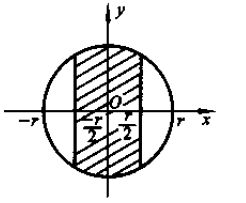
\includegraphics[width=0.4\textwidth]{fig3-1-4.png}
\caption{$p(x,y)$ 的非零区域与有关事件的交集部分}\label{fig:3.1.4}
\end{figure}

\textbf{四、二元正态分布}

如果二维随机变量 $(X,Y)$ 的联合密度函数 (见图~\ref{fig:3.1.5}) 为
	\begin{equation}\label{eq:3.1.8}
	\begin{aligned} 
	p(x, y) &=\frac{1}{2 \pi \sigma_{1} \sigma_{2} \sqrt{1-\rho^{2}}} \exp \bigg\{-\frac{1}{2\left(1-\rho^{2}\right)}
	\bigg[\frac{\left(x-\mu_{1}\right)^{2}}{\sigma_{1}^{2}}		\\
	&-2 \rho \frac{\left(x-\mu_{1}\right)\left(y-\mu_{2}\right)}{\sigma_{1} \sigma_{2}}+\frac{\left(y-\mu_{2}\right)^{2}}{\sigma_{2}^{2}} 
	\bigg] \bigg\}, \quad-\infty<x, y<+\infty \\
	\end{aligned}
	\end{equation}
则称 $(X,Y)$ 服从二元正态分布, 记为 $(X,Y)\sim N(\mu_1,\mu_2,\sigma_1^2,\sigma_2^2,\rho)$. 其中五个参数的取值范围分别是:
	\[
	 	-\infty<\mu_{1}, \mu_{2}<+\infty; \quad \sigma_{1}, \sigma_{2}>0 ; \quad-1 \leq \rho \leq 1.
	\]
	以后将指出: $\mu_1,\mu_2$ 分别是 $X$ 与 $Y$ 的均值, $\sigma_1^2,\sigma_2^2$ 分别是 $X$ 与 $Y$ 的方差, $\rho$ 是
	 $X$ 与 $Y$ 的相关系数.

	 二元正态密度函数的图形很像一顶四周无限延伸的草帽, 其中心点在 $(\mu_1,\mu_2)$ 处, 其等高线是椭圆.

	 \begin{figure}[htbp]
	 	\centering
	 	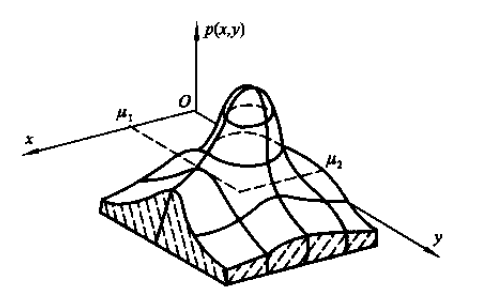
\includegraphics[width=0.4\textwidth]{fig3-1-5.png}
	 	\caption{二元正态密度函数}\label{fig:3.1.5}
	 \end{figure}

	 \begin{example}\label{exam:3.1.7}
	 	设二维随机变量 $(X,Y)\sim N(\mu_1,\mu_2,\sigma_1^2,\sigma_2^2,\rho)$, 求 $(x,Y)$ 落在区域
	 	\[
	 	 	D=\left\{(x, y) ; \frac{\left(x-\mu_{1}\right)^{2}}{\sigma_{1}^{2}}-2 \rho \frac{\left(x-\mu_{1}\right)\left(y-\mu_{2}\right)}{\sigma_{1} \sigma_{2}}+\frac{\left(y-\mu_{2}\right)^{2}}{\sigma_{2}^{2}} \leqslant \lambda^{2}\right\}
	 	\]
	 	内的概率.
	 \end{example}
	 \begin{solution}
	 	所求的概率为
	 	\begin{equation*}
			\begin{aligned} 
			p(x, y) &=\frac{1}{2 \pi \sigma_{1} \sigma_{2} \sqrt{1-\rho^{2}}} \iint_D \exp \bigg\{-\frac{1}{2\left(1-\rho^{2}\right)}
			\bigg[\frac{\left(x-\mu_{1}\right)^{2}}{\sigma_{1}^{2}}		\\
			&-2 \rho \frac{\left(x-\mu_{1}\right)\left(y-\mu_{2}\right)}{\sigma_{1} \sigma_{2}}+\frac{\left(y-\mu_{2}\right)^{2}}{\sigma_{2}^{2}} 
			\bigg] \bigg\} \dd x \dd y\\
			\end{aligned}
		\end{equation*}
		作变换
		\[
		 	\begin{cases}
		 		u =\frac{x-\mu_1}{\sigma_1}-\rho \frac{y-\mu_2}{\sigma_2},\\
		 		v =\frac{y-\mu_2}{\sigma_2}\sqrt{1-\rho^2}.
		 	\end{cases}
		\]
		则可得
		\[
		 	\frac{\partial(u, v)}{\partial(x, y)}= \begin{vmatrix}{\frac{1}{\sigma_{1}}} & {0} \\ {-\frac{\rho}{\sigma_{2}}} & {\frac{\sqrt{1-\rho^{2}}}{\sigma_{2}}}\end{vmatrix}=\frac{\sqrt{1-\rho^{2}}}{\sigma_{1} \sigma_{2}}, \quad|J|=\frac{\sigma_{1} \sigma_{2}}{\sqrt{1-\rho^{2}}},
		\]
		由此得
		\[
		 	p=\frac{1}{2 \pi(1-\rho^{2})} \iint_{x^{2}+v^{2} \leq \lambda^{2}} \exp \left\{-\frac{u^{2}+v^{2}}{2\left(1-\rho^{2}\right)}\right\} \dd u \dd v
		\]
		再作极坐标变换
		\[
		 	\begin{cases} 
		 		u=r \sin \alpha ,\\ 
		 		v=r \cos \alpha	,
		 	\end{cases}
		\]
		则可得
		\[
		 	J=\frac{\partial(u, v)}{\partial(r, \alpha)}= \begin{vmatrix}{\sin \alpha} & {\cos \alpha} \\ {r \cos \alpha} & {-r \sin \alpha}\end{vmatrix}=-r\left(\sin ^{2} \alpha+\cos ^{2} \alpha\right)=-r,
		\]
		最后得
		\[
		 	\begin{aligned} 
		 	p &=\frac{1}{2 \pi (1-\rho^{2})} \int_{0}^{2 \pi} \dd \alpha \int_{0}^{\lambda} r \exp \left\{-\frac{r^{2}}{2\left(1-\rho^{2}\right)}\right\} \dd r \\ 
		 	&=\int_{0}^{\lambda} \exp \left\{-\frac{r^{2}}{2\left(1-\rho^{2}\right)}\right\}\dd \left(\frac{r^{2}}{2\left(1-\rho^{2}\right)}\right)\\ 
		 	&=\left.-\exp \left\{-\frac{r^{2}}{2\left(1-\rho^{2}\right)}\right\}\right|_{0} ^{\lambda}=1-\exp \left\{-\frac{\lambda^{2}}{2\left(1-\rho^{2}\right)}\right\} .
		 	\end{aligned}
		\]
	 \end{solution}

	 \begin{xiti}
	 	\item 一批产品中有一等品 50\%, 二等品 30\%, 三等品 20\%. 从中有放回地抽取 5 件, 以 $X$、$Y$ 分别表示取出的 5 件中一等品、二等品的件数, 
	 	求 $(X,Y)$ 的联合分布列.
	 	\item 100 件产品中有 50 件一等品, 30 件二等品, 20 件三等品. 从中不放回地抽取 5 件, 以 $X$、$Y$ 分别表示取出的 5 件中一等品、二等品的件数,
	 	求 $(X,Y)$ 的联合分布列.
	 	\item 盘子里装有 3 只黑球、2 只红球、2 只白球, 从中任取 4 只, 以 $X$ 表示取到黑球的只数, 以 $Y$ 表示取到红球的只数,试求 $P\{X=Y\}$.
	 	\item 设随机变量 $X_i$,$i=1,2$, 的分布列如下, 且满足 $P(X_1X_2=0) =1$, 试求 $P(X_1=X_2)$.
	 	\begin{center}
	 		\begin{tabularx}{0.8\textwidth}{Z|ZZZ}
	 		$X_t$&	-1&		0&		1	\\
	 		\hline
	 		$P$	&	0.25&	0.5&	0.25	\\
	 	\end{tabularx}
	 	\end{center}
	 	\item 设随机变量 $(X,Y)$ 的联合密度函数为
	 	\[
	 	 	p(x, y)=\begin{cases}k(6-x-y),\quad & 0<x<2,2<y<4 \\
	 	 	 0,				&	\text{其他} .
	 	 	\end{cases}
	 	\]
	 	试求
	 	\begin{enumerate}[(1)]
	 		\item 常数 $k$;
	 		\item $P\{X<1,Y<3\}$;
	 		\item $P\{X<1.5\}$;
	 		\item $P\{X+Y\leq 4\}$.
	 	\end{enumerate}
	 	\item 设随机变量 $(X,Y)$ 的联合密度函数为
	 	\[
	 	 	p(x, y)=\begin{cases}
	 	 				k \ee^{-(3 x+4 y)},&	x>0,y>0 \\
	 	 	 			0,		&		\text{其他} . 
	 	 	 		\end{cases}
	 	\]
	 	试求
	 	\begin{enumerate}[(1)]
	 		\item 常数 $k$;
	 		\item $(X,Y)$ 的联合分布函数 $F(X,Y)$;
	 		\item $P\{0<X\leq 1,0<Y\leq 2\}$.
	 	\end{enumerate}
	 	\item 设二维随机变量 $(X,Y)$ 的联合密度函数为
	 	\[
	 	 	p(x, y)=\begin{cases}
	 	 				4 x y,&	0<x<1,0<y<1, \\ 
	 	 				0,&		\text{其他} .
	 	 			\end{cases}
	 	\]
	 	试求
	 	\begin{enumerate}[(1)]
	 		\item $P(0<X<0.5,0.25<Y<1)$;
	 		\item $P(X+Y)$;
	 		\item $P(X<Y)$;
	 		\item $(X,Y)$ 的联合分布函数.
	 	\end{enumerate}
	 	\item 设二维随机变量 $(X,Y)$ 的联合密度函数为
	 	\[
	 	 	p(x,y)=\begin{cases}
	 	 		k,&		0<x^2<y<x<1;\\
	 	 		0,&		\text{其他} .
	 	 	\end{cases}
	 	\]
	 	\begin{enumerate}[(1)]
	 		\item 试求常数 $k$;
	 		\item 求 $P(X>0.5)$ 和 $P(Y<0.5)$. 
	 	\end{enumerate}
	 	\item 设二维随机变量 $(X,Y)$ 的联合密度函数为
	 	\[
	 	 	p(x,y)=\begin{cases}
	 	 		6 (1-y),&	0<x<y<1;	\\
	 	 		0,&			\text{其他} .
	 	 	\end{cases}
	 	\]
	 	\begin{enumerate}[(1)]
	 		\item 求 $P(X>0.5,Y>0.5)$;
	 		\item 求 $P(X<0.5)$ 和 $P(Y<0.5)$;
	 		\item 求 $P(X+Y)<1$.
	 	\end{enumerate}
	 	\item 设随机变量 $Y$ 服从参数为 $\lambda=1$ 的指数分布, 定义随机变量 $X_k$ 如下
	 	\[
	 	 	X_k=\begin{cases}
	 	 		0,&		Y\leq k, \\
	 	 		1,&		Y>k,
	 	 	\end{cases} \quad k=1,2.
	 	\]
	 	求 $X_1$ 和 $X_2$ 的联合分布列.
	 	\item 设二维随机变量 $(X,Y)$ 的联合密度函数为
	 	\[
	 	 	p(x,y)=\begin{cases}
	 	 		x^2+\frac{xy}{3},&	0<x<1,0<y<2;\\
	 	 		0,		&			\text{其他} .
	 	 	\end{cases}
	 	\]
	 	求 $P(X+Y)\geq 1$.
	 	\item 设二维随机变量 $(X,Y)$ 的联合密度函数为
	 	\[
	 	 	p(x,y)=\begin{cases}
	 	 		\ee^{-y},	&	0<x<y;\\
	 	 		0&			\text{其他} .
	 	 	\end{cases}
	 	\]
	 	试求 $P(X,Y)\leq 1$.
	 	\item 设二维随机变量 $(X,Y)$ 的联合密度函数为
	 	\[
	 	 	p(x,y)=\begin{cases}
	 	 		1/2,&	0<x<1,0<y<2;\\
	 	 		0,&		\text{其他} .	
	 	 	\end{cases}
	 	\]
	 	求 $X$ 与 $Y$ 中至少一个小于 0.5 的概率.
	 	\item 从 (0,1) 中随机地取两个数, 求其积不小于 3/16, 且其和不大于 1 的概率.
	 \end{xiti}

	\section{边际分布与随机变量的独立性}\label{sec:3.2}
  二维联合分布函数(二维联合分布列、二维联合密度函数也一样)含有丰富的信息,\ 主要有以下三方面信息:
  \begin{itemize}
  	\item 每个分量的分布(每个分量的所有信息),\ 即边际分布.
  	\item 两个分量之间的关联程度,\ 即协方差和相关系数.
  	\item 给定一个分量时,\ 另一个分量的分布,\ 即条件分布.
  \end{itemize}
  我们的目的时将这些信息从联合分布中挖掘出来,\ 本节先讨论边际分布.
  
  \subsection{边际分布函数}\label{ssec:3.2.1}
  如果在二维随机变量 $(X,Y)$ 的联合分布函数 $F(X,Y)$ 中令 $y\to+\infty$ ,\ 由于 $|Y<+\infty|$ 为必然事件,\ 故可得
  \begin{equation*}
  \lim_{y\to+\infty}F(x,y)=P(X\leqslant x,Y<+\infty)=P(X\leqslant x),
  \end{equation*}
  这是一个分布函数,\ 被称为 $X$ 的边际分布,\ 记为
  \begin{equation}
  F_{X}(x)=F(x,+\infty).\label{eq:3.2.1}
  \end{equation}
  类似地,\ 在 $F(x,y)$ 中令 $x\to+\infty$ ,\ 可得 $Y$ 的边际分布
  \begin{equation}
  F_{Y}(y)=F(+\infty,y).\label{eq:3.2.2}
  \end{equation}
  在三维随机变量 $(X,Y,Z)$ 的联合分布函数 $F(x,y,z)$ 中,\ 用类似的方法可得到更多的边际分布函数:
  \begin{align*}
  &F_{X}(x) = F(x,+\infty,+\infty);\\
  &F_{Y}(y) = F(+\infty,y,+\infty);\\
  &F_{Z}(z) = F(+\infty,+\infty,z);\\
  &F_{X,Y}(x,y) = F(x,y,+\infty);\\
  &F_{X,Z}(x,z) = F(x,+\infty,z);\\
  &F_{Y,Z}(y,z) = F(+\infty,y,z).
  \end{align*}
  在更高维的场合,\ 也可类似地从联合分布函数获得其低维的边际分布函数.
  \begin{example}\label{exam:3.2.1}
  	设二维随机变量 $(X,Y)$ 的联合分布函数为
  	\begin{equation*}
  	F(x,y)=
  	\begin{cases}
  	1-\ee^{-x}-\ee^{-y}+\ee^{-x-y-\lambda xy}, & x>0,y>0;\\
  	0, & \text{其他}.
  	\end{cases}
  	\end{equation*}
  	这个分布被称为二维指数分布,\ 其中参数 $\lambda>0$.
  	
  	由此联合分布函数 $F(x,y)$ ,\ 容易获得 $X$ 与 $Y$ 的边际分布函数为
  	\begin{align*}
  	F_{X}(x) &= F(x,+\infty)=
  	\begin{cases}
  	1-\ee^{-x}, & x>0;\\
  	0, & x\leqslant0.
  	\end{cases}\\
  	F_{Y}(y) &= F(+\infty,y)=
  	\begin{cases}
  	1-\ee^{-y}, & y>0;\\
  	0, & y\leqslant0.
  	\end{cases}
  	\end{align*}
  	它们都是一维指数分布,\ 且与参数 $\lambda>0$ 无关.\ 不同的 $\lambda>0$ 对应不同的二维指数分布,\ 但它们的两个边际分布不变.\ 这说明:\ 二维联合分布不仅含有每个分量的概率分布,\ 而且还含有两个变量 $X$ 与 $Y$ 间关系的信息,\ 这正是人们要研究多维随机变量的原因.
  \end{example}
  
  \subsection{边际分布列}\label{ssec:3.2.2}
  在二维离散随机变量 $(X,Y)$ 的联合分布列 $\left\{P(X=x_i,Y=y_i)\right\}$ 中,\ 对 $j$ 求和所得的分布列
  \begin{equation}
  \sum_{j=1}^{+\infty}P(X=x_i,Y=y_j)=P(X=x_i),\ i=1,2,\ldots\label{eq:3.2.3}
  \end{equation}
  被称为 $X$ 的边际分布列.\ 类似地,\ 对 $i$ 求和所得的分布列
  \begin{equation}
  \sum_{i=1}^{+\infty}P(X=x_i,Y=y_j)=P(Y=y_j),\ j=1,2,\ldots\label{eq:3.2.4}
  \end{equation}
  被称为 $Y$ 的边际分布列.
  \begin{example}\label{exam:3.2.2}
  	设二维随机变量 $(X,Y)$ 有如下的联合分布列
  	\begin{equation*}
  	\begin{tabularx}{0.8\textwidth}{ZZZZ}
  	\toprule
  	 & \multicolumn{3}{c}{$Y$}\\
  	\cmidrule{2-4}
  	$X$ & 1 & 2 & 3\\
  	\midrule
  	0 & 0.09 & 0.21 & 0.24\\
  	1 & 0.07 & 0.12 & 0.27\\
  	\bottomrule
  	\end{tabularx}
  	\end{equation*}
  	求 $X$ 与 $Y$ 的边际分布列.
  	\end{example}
  
  \begin{solution}
  	在上述联合分布列中,\ 对每一行求和得 $0.54$ 与 $0.46$ ,\ 并把它们写在对应行得右侧,\ 这就是 $X$ 的边际分布列.\ 再对每一列求和,\ 得 $0.16,0.33$ 和 $0.51$ ,\ 并把它们写在对应列的下侧,\ 这就是 $Y$ 得边际分布列.
  	\begin{equation*}
  	\begin{tabularx}{0.8\textwidth}{ZZZZZ}
  	\toprule
  	 & \multicolumn{3}{c}{$Y$} & \\
  	 \cmidrule{2-4}
  	$X$ & 1 & 2 & 3 & $P(X=i)$ \\
  	\midrule
  	0 & 0.09 & 0.21 & 0.24 & 0.54 \\
  	1 & 0.07 & 0.12 & 0.27 & 0.46 \\
  	\midrule
  	$P(Y=j)$ & 0.16 & 0.33 & 0.51 &1\\
  	\bottomrule
  	\end{tabularx}
  	\end{equation*}
  \end{solution}

  \subsection{边际密度函数}\label{ssec:3.2.3}
  如果二维连续随机变量 $(X,Y)$ 的联合密度函数为 $p(x,y)$ ,\ 因为
  \begin{align*}
  F_{X}(x) &= F(x,+\infty)=\int_{-\infty}^{x}\left( \int_{-\infty}^{+\infty}p(u,v)\,\dd v \right)\,\dd u=\int_{-\infty}^{x}p_{X}(u)\,\dd u,\\
  F_{Y}(y) &= F(+\infty,y)=\int_{-\infty}^{y}\left( \int_{-\infty}^{+\infty}p(u,v)\,\dd u \right)\,\dd v=\int_{-\infty}^{y}p_{Y}(v)\,\dd v,
  \end{align*}
  其中 $p_{X}(x)$ 和 $p_{Y}(y)$ 分别为
  \begin{align}
  p_{X}(x) &= \int_{-\infty}^{+\infty}p(x,y)\,\dd y.\label{eq:3.2.5}\\
  p_{Y}(y) &= \int_{-\infty}^{+\infty}p(x,y)\,\dd x.\label{eq:3.2.6}
  \end{align}
  它们恰好处于密度函数位置,\ 故称上式给出的 $p_{X}(x)$ 为 $X$ 的边际密度函数,\ $p_{Y}(y)$ 为 $Y$ 的边际密度函数.
  
  由联合密度函数求边际密度函数时,\ 要注意积分区域的确定.
  \begin{example}\label{exam:3.2.3}
  	设二维随机变量 $(X,Y)$ 的联合密度函数为
  	\begin{equation*}
  	p(x,y)=
  	\begin{cases}
  	1, & 0<x<1,|y|<x;\\
  	0, & \text{其他}.
  	\end{cases}
  	\end{equation*}
  	试求:(1)边际密度函数 $p_{X}(x)$ 和 $p_{Y}(y)$;(2) $P(X<1/2)$ 及 $P(Y>1/2)$ .
  \end{example}
  \begin{solution}
  	首先识别 $p(x,y)$ 的非零区域,\ 它如图~\ref{fig:3.2.1} 所示.
  	\begin{figure}[htbp]
  		\centering
  		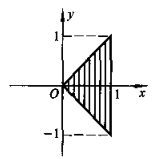
\includegraphics[scale=0.5]{fig3-2-1.png}
  		\caption{$p(x,y)$ 的非零区域}\label{fig:3.2.1}
  	\end{figure}
  	\begin{itemize}
  		\item[(1)]求 $p_X(x)$:\ 当 $x\leqslant0$ 或 $x\geqslant1$ 时,\ 有 $p_X(x)=0$.\ 而当 $0<x<1$ 时,\ 有
  		\begin{equation*}
  		p_X(x)=\int_{-\infty}^{+\infty}p(x,y)\,\dd y=\int_{-x}^{x}\,\dd y=2x.
  		\end{equation*}
  		所以 $X$ 的边际密度函数为(见图~\ref{fig:3.2.2})
  		\begin{equation*}
  		p_X(x)=
  		\begin{cases}
  		2x, & 0<x<1;\\
  		0, & \text{其他}.
  		\end{cases}
  		\end{equation*}
  		\begin{figure}[h]
  			\centering
  			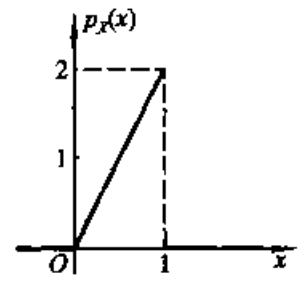
\includegraphics[scale=0.2]{fig3-2-2.png}
  			\caption{$X$ 的边际密度函数}\label{fig:3.2.2}
  		\end{figure}
  		再求 $p_Y(y):$\ 当 $y\leqslant-1$ 或 $y\geqslant1$ 时,\ 有 $p_Y(y)=0$.\ 而当 $-1<y<0$ 时,\ 有
  		\begin{equation*}
  		p_Y(y)=\int_{-\infty}^{+\infty}p(x,y)\,\dd x=\int_{-y}^{1}\,\dd x=1+y,
  		\end{equation*}
  		当 $0<y<1$ 时,\ 有
  		\begin{equation*}
  		p_Y(y)=\int_{-\infty}^{+\infty}p(x,y)\,\dd x=\int_{y}^{1}\,\dd x=1-y.
  		\end{equation*}
  		所以 $Y$ 的边际密度函数为(见图~\ref{fig:3.2.3})
  		\begin{equation*}
  		p_{Y}(y)=
  		\begin{cases}
  		1+y, & -1<y<0,\\
  		1-y, & 0<y<1,\\
  		0, & \text{其他}.
  		\end{cases}
  		\end{equation*}
  		\begin{figure}[h]
  			\centering
  			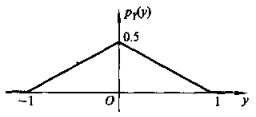
\includegraphics[scale=0.5]{fig3-2-3.png}
  			\caption{ $Y$ 的边际密度函数}\label{fig:3.2.3}
  		\end{figure}
  		\item[(2)] 要求的概率分别为
  		\begin{align*}
  		P(X<1/2) &= \int_{-\infty}^{1/2}p_{X}(x)\,\dd x=\int_{0}^{1/2}2x\,\dd x=\frac{1}{4}.\\
  		P(Y>1/2) &= \int_{1/2}^{+\infty}p_{Y}(y)\,\dd y=\int_{1/2}^{1}(1-y)\,\dd y=\frac{1}{8}.
  		\end{align*}
  	\end{itemize}
  \end{solution}
  
  \begin{example}\label{exam:3.2.4}
  	多项分布的边际分布仍为多项分布
  \end{example}
  \begin{solution}
  	下面只证三项分布的边际分布为二项分布.\ 设 $(X,Y)$ 服从三项分布 $M(n,p_1,p_2,p_3),$ \ 其联合分布列为
  	\begin{equation*}
  	P(X=i,Y=j)=\frac{n!}{i!j!(n-i-j)!}p_1^ip_2^j(1-p_1-p_2)^{n-i-j},\ i,j=1,2,\ldots,n,i+j\leqslant n.
  	\end{equation*}
  	对上式分别乘以和除以 $(1-p_1)^{n-i}/(n-i)!$ ,\ 再对 $j$ 从 $0$ 到 $n-1$ 求和,\ 并记 $p_2'=p_2/(1-p_1)$,\ 则可得
  	\begin{align*}
  	&\sum_{j=0}^{n-i}P(X=i,Y=j) = \frac{n!}{i!(n-i)!}p_1^i(1-p_1)^{n-i}.\\
  	&\sum_{j=0}^{n-i} \binom{n-i}{j} \left(\frac{p_2}{1-p_1}\right)^{j}\left(1-\frac{p_2}{1-p_1}\right)^{n-i-j} \\
  	&= \frac{n!}{i!(n-i)!}p_1^i(1-p_1)^{n-i}\left[p_2'+(1-p_2')\right]^{n-i}\\
  	&= \frac{n!}{i!(n-i)!}p_1^i(1-p_1)^{n-i}.
  	\end{align*}
  	所以 $X\sim b(n,p_1)$ .\ 同理可证 $Y\sim b(n,p_2)$.
  	
  	用类似的方法可以证明:\ 若 $(X_,,X_2,\ldots,X_r)\sim M(n,p_1,p_2,\ldots,p_r)$,\ 则 $X_i\sim b(n,p_i),\ i=1,2,\ldots,r$.
  \end{solution}
  
  \begin{example}\label{exam:3.2.5}
  	二维正态分布的边际分布为一维正态分布
  \end{example}
  \begin{solution}
  	设 $(X,Y)\sim N(\mu_1,\mu_2,\sigma_1^2,\sigma_2^2,\rho)$ .\ 先把 ~\ref{eq:3.1.8} 式二维正态密度函数 $p(x,y)$ 的指数部分
  	\begin{equation*}
  	-\frac{1}{2(1-\rho^2)}\left[\frac{(x-\mu_1)^2}{\sigma_1^2}-2\rho\frac{(x-\mu_1)(y-\mu_2)}{\sigma_1\sigma_2}+\frac{(y-\mu_2)^2}{\sigma_2^2}\right]
  	\end{equation*}
  	改写成
  	\begin{equation*}
  	-\frac{1}{2}\left[\rho\frac{x-\mu_1}{\sigma_1\sqrt{1-\rho^2}}-\frac{y-\mu_2}{\sigma_2\sqrt{1-\rho^2}}\right]^2-\frac{(x-\mu_1)^2}{2\sigma_1^2}.
  	\end{equation*}
  	再对积分
  	\begin{equation*}
  	\int_{-\infty}^{+\infty}\exp\left\{-\frac{1}{2}\left[\rho\frac{x-\mu_1}{\sigma_1\sqrt{1-\rho^2}}-\frac{y-\mu_2}{\sigma_2\sqrt{1-\rho^2}}\right]^2\right\}\,\dd y
  	\end{equation*}
  	作变换(注意把 $x$ 看作常量)
  	\begin{equation*}
  	t=\rho\frac{x-\mu_1}{\sigma_1\sqrt{1-\rho^2}}-\frac{y-\mu_2}{\sigma_2\sqrt{1-\rho^2}},
  	\end{equation*}
  	则
  	\begin{align*}
  	p_{X}(x) &= \int_{-\infty}^{+\infty}p(x,y)\,\dd y\\
  	&=\frac{1}{2\uppi\sigma_1\sigma_2\sqrt{1-\rho^2}}\exp\left\{-\frac{(x-\mu_1)^2}{2\sigma_1^2}\right\}\sigma_2\sqrt{1-\rho^2}\int_{-\infty}^{+\infty}\exp\left\{-\frac{t^2}{2}\right\}\,\dd t.
  	\end{align*}
  	注意到上式中的积分恰好等于 $\sqrt{2\uppi}$ ,\ 所以有
  	\begin{equation*}
  	p_{X}(x)=\frac{1}{\sqrt{2\uppi}\sigma_1}\exp\left\{-\frac{(x-\mu_1)^2}{2\sigma_1^2}\right\}.
  	\end{equation*}
  	这正是一维正态分布 $N(\mu_1,\sigma_1^2)$ 的密度函数,\ 即 $X\sim N(\mu_1,\sigma_1^2)$ .\ 同理可证 $Y\sim N(\mu_2,\sigma_2^2)$ .\ 由此可见
  	\begin{itemize}
  		\item 二维正态分布的边际分布中不含参数 $\rho$ .
  		\item 这说明二维正态分布 $N(\mu_1,\mu_2,\sigma_1^2,\sigma_2^2,0.1)$ 与 $N(\mu_1,\mu_2,\sigma_1^2,\sigma_2^2,0.2)$ 的边际分布是相同的.
  		\item 具有相同边际分布的多维联合分布可以是不同的.
  	\end{itemize}
  \end{solution}
  
   \subsection{随机变量间的独立性}\label{ssec:3.2.4}
   在多维随机变量中,\ 各分量的取值有时会相互影响,\ 但有时毫无影响.\ 譬如一个人的身高 $X$ 和体重 $Y$ 就会相互影响,\ 但与收入 $Z$ 一般无影响.\ 当两个随机变量取值的规律互不影响时,\ 就称它们是相互独立的.
   \begin{definition}{}{3.2.1}
   	设 $n$ 维随机变量 $(X_1,X_2,\ldots,X_n)$ 的联合分布函数为 $F(x_1,x_2,\ldots,x_n)$ ,\ $F_i(x_i)$ 为 $X_i$ 的边际分布函数.\ 如果对任意 $n$ 个实数 $x_1,x_2,\ldots,x_n$ ,\ 有
   	\begin{equation}\label{eq:3.2.7}
   		F(x_1,x_2,\ldots,x_n)=\prod_{i=1}^{n}F_i(x_i),
   	\end{equation}
   	则称 $X_1,X_2,\ldots,X_n$ 相互独立.
   \end{definition}
   在离散随机变量场合,\ 如果对其任意 $n$ 个取值 $x_1,x_2,\ldots,x_n$ ,\ 有
   \begin{equation}\label{eq:3.2.8}
   	P(X_1=x_1,X_2=x_2,\ldots,X_n=x_n)=\prod_{i=1}^{n}P(X_i=x_i),
   \end{equation}
   则称 $X_1,X_2,\ldots,X_n$ 相互独立.
   
   在连续随机变量场合,\ 如果对任意 $n$ 个实数 $x_1,x_2,\ldots,x_n$ ,\ 有
   \begin{equation}\label{eq:3.2.9}
   	p(x_1,x_2,\ldots,x_n)=\prod_{i=1}^{n}p_i(x_i),
   \end{equation}
   则称 $X_1,X_2,\ldots,X_n$ 相互独立.
   
   \begin{example}
   	设 $(X,Y)$ 是二维离散随机变量,\ $X$ 和 $Y$ 的边际分布列分别如下所示:
   	\begin{table}[h]
   		\centering
   		\begin{tabularx}{0.4\textwidth}{Z|ZZZ}
   			\hline
   			$X$ & $-1$ & $0$ & $1$\\
   			\hline
   			$P$ & $1/4$ & $1/2$ & $1/4$\\
   			\hline
   		\end{tabularx}
   	    \qquad
   	    \begin{tabularx}{0.4\textwidth}{Z|ZZ}
   	    	\hline
   	    	$Y$ & $0$ & $1$\\
   	    	\hline
   	    	$P$ & $1/2$ & $1/2$\\
   	    	\hline
   	    \end{tabularx}
   	\end{table}
   如果 $P\left\{XY=0\right\}=1$,\ 试求
   
   (1) $(X,Y)$ 的联合分布列;
   
   (2) $X$ 与 $Y$ 是否独立?

   \end{example}
   \begin{solution}
   	\begin{itemize}
   		\item[(1)] 记 $(X,Y)$ 得联合分布列如下,\ 其中 $p_{ij}=P(X=i,Y=j)$ ,\ 在联合分布列的右侧是 $X$ 的边际分布列,\ 下侧是 $Y$ 的边际分布列.
   		\begin{center}
   			\begin{tabularx}{0.8\textwidth}{XXXX}
   				\toprule
   				 & \multicolumn{2}{c}{$Y$} & \\
   				\cmidrule{2-3}
   				$X$ & $0$ & $1$ & $P(X=i)$\\
   				\midrule
   				$-1$ & $p_{11}$ & $p_{12}$ & $1/4$\\
   				$0$ & $p_{21}$ & $p_{22}$ & $1/2$\\
   				$1$ & $p_{31}$ & $p_{32}$ & $1/4$\\
   				\midrule
   				$P(Y=j)$ & $1/2$ & $1/2$ & $1$\\
   				\bottomrule
   			\end{tabularx}
   		\end{center}
   		由 $P(XY=0)=1$ ,\ 知 $P(XY\ne0)=0$ ,\ 即
   		\begin{equation*}
   		p_{12}=P(X=-1,Y=1)=0,\quad p_{32}=P(X=1,Y=1)=0.
   		\end{equation*}
   		其余四个概率可由下面等式分别确定.
   		\begin{center}
   			\begin{tabular}{l}
   				从表中第一行看,\ 由 $p_{11}+p_{12}=1/4$ ,\ 得 $p_{11}=1/4$ .\\
   				从表中第三行看,\ 由 $p_{31}+p_{32}=1/4$ ,\ 得 $p_{31}=1/4$ .\\
   				从表中第一列看,\ 由 $p_{11}+p_{21}+p_{31}=1/2=1/4+p_{21}+1/4$ ,\ 得 $p_{21}=0$ .\\
   				从表中第二列看,\ 由 $p_{12}+p_{22}+p_{32}=1/2=0+p_{22}+0$ ,\ 得 $p_{22}=1/2$ .
   			\end{tabular}
   		\end{center}
   		
   		于是得 $(X,Y)$ 的联合分布列如下:
   		\begin{center}
   			\begin{tabularx}{0.8\textwidth}{XXXX}
   				\toprule
   				 & \multicolumn{2}{c}{$Y$} & \\
   				\cmidrule{2-3}
   				$X$ & 0 & 1 & $p_{i\cdot}$\\
   				\midrule
   				$-1$ & $1/4$ & $0$ & $1/4$\\
   				$0$ & $0$ & $1/2$ & $1/2$\\
   				$1$ & $1/4$ & $0$ & $1/4$\\
   				\midrule
   				$p_{\cdot j}$ & $1/2$ & $1/2$ & $1$\\
   				\bottomrule
   			\end{tabularx}
   		\end{center}
   		\item[(2)] 因为 $P(X=0,Y=0)=p_{21}=0$ ,\ 而 $P(X=0)P(Y=0)=1/4$ ,\ 所以 $X$ 与 $Y$ 不独立.
   	\end{itemize}
   \end{solution}

   \begin{example}\label{exam:3.2.7}
   	若 $(X,Y)$ 的联合密度函数为
   	\begin{equation*}
   		p(x,y)=
   		\begin{cases}
   		8xy, & 0\leqslant x\leqslant y\leqslant1;\\
   		0, & \text{其他}.
   		\end{cases}
   	\end{equation*}
   	问 $X$ 与 $Y$ 是否相互独立?
   \end{example}
   \begin{solution}
   	为判断 $X$ 与 $Y$ 是否独立,\ 只需看边际密度函数的乘积是否等于联合密度函数.\ 为此先求边际密度函数.
   	当 $x<0$ 或 $x>1$ 时,\ $p_{X}(x)=0$ .\ 而当 $0\leqslant x\leqslant1$ 时,\ 有
   	\begin{equation*}
   		p_{X}(x)=\int_{x}^{1}8xy\,\dd y=8x\left(\frac{1}{2}-\frac{x^2}{2}\right)=4x\left(1-x^2\right).
   	\end{equation*}
   	因此
   	\begin{equation*}
   		p_{X}(x)=
   		\begin{cases}
   		4x\left(1-x^2\right), & 0\leqslant x\leqslant1,\\
   		0, & \text{其他}.
   		\end{cases}
   	\end{equation*}
   	同样,\ 当 $y<0$ 或 $y>1$ 时,\ $p_{Y}(y)=0$ .\ 而当 $0\leqslant y\leqslant 1$ 时,\ 有
   	\begin{equation*}
   		p_{Y}(y)=\int_{0}^{x}8xy\,\dd x=4y^3.
   	\end{equation*}
   	因此
   	\begin{equation*}
   		p_{Y}(y)=
   		\begin{cases}
   		4y^3, & 0\leqslant y\leqslant1;\\
   		0, & \text{其他}.
   		\end{cases}
   	\end{equation*}
   	由此得 $p(x,y)\ne p_{X}(x)p_{Y}(y)$ ,\ 所以 $X$ 与 $Y$ 不独立.
   \end{solution}

   \begin{example}\label{exam:3.2.8}
   	从 $(0,1)$ 中任取两个数,\ 求下列事件的概率.
   	
   	(1)两数之和小于 $1.2$ ;
   	
   	(2)两数之积小于 $1/4$ .
   \end{example}
   \begin{solution}
   	分别记这两个数为 $X$ 和 $Y$ ,\ 则 $X$ 和 $Y$ 独立,\ 且都服从 $(0,1)$ 上的均匀分布,\ $(X,Y)$ 的联合密度函数为
   	\begin{equation*}
   		p(x,y)=p_{X}(x)p_{Y}(y)=
   		\begin{cases}
   		1, & 0<x<1,0<y<1;\\
   		0, & \text{其他}.
   		\end{cases}
   	\end{equation*}
   	\begin{itemize}
   		\item[(1)] 从图~\ref{fig:3.2.4a}可知
   		\begin{align*}
   			P(X+Y<1.2)=\int_{0}^{0.2}\int_{0}^{1}\,\dd y\dd x+\int_{0.2}^{1}\int_{0}^{1.2-x}\,\dd y\dd x\\
   			=0.2+\int_{0.2}^{1}(1.2-x)\,\dd x=0.2+0.48=0.68\ .
   		\end{align*}
   		\begin{figure}[h]
   			\centering
   			\subfloat[$\{x+y<1.2,0<x,y<1\}$]{\label{fig:3.2.4a}
   			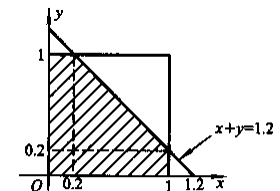
\includegraphics[scale=0.5]{fig3-2-4a.png}}
   			\qquad
   			\subfloat[$\{xy<1/4,0<x,y<1\}$]{\label{fig:3.2.4b}
   			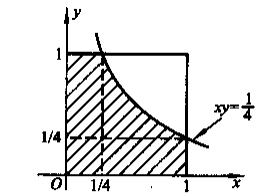
\includegraphics[scale=0.5]{fig3-2-4b.png}
   			}
   			\caption{ $p(x,y)$ 的非零区域与有关事件的交集部分}\label{fig:3.2.4}
   		\end{figure}
   	\item[(2)] 从图~\ref{fig:3.2.4b}可知
   	\begin{align*}
   		P(XY<1/4)=\int_{0}^{1/4}\int_{0}^{1}\,\dd y\dd x+\int_{1/4}^{1}\int_{0}^{1/(4x)}\,\dd y\dd x\\
   		=\frac{1}{4}+\int_{1/4}^{1}\frac{1}{4x}\,\dd x=\frac{1}{4}+\frac{1}{4}\ln4=0.5966\ .
   	\end{align*}
   	\end{itemize}
   \end{solution}

   \begin{xiti}
   		\item 设二维离散随机变量 $(X,Y)$ 的可能值为
   		\begin{equation*}
   			(0,0),\ (-1,1),\ (-1,2),\ (1,0).
   		\end{equation*}
   		且取这些值的概率依次为 $1/6,1/3,1/12,5/12$ ,\ 试求 $X$ 与 $Y$ 各自的边际分布列.
   		\item 设二维随机变量 $(X,Y)$ 的联合分布函数为
   		\begin{equation*}
   			F(x,y)=\begin{cases}
   			1-\ee^{-\lambda_{1}x}-\ee^{-\lambda_{2}y}+\ee^{-\lambda_{1}x-\lambda_{2}y-\lambda_{12}\max\{x,y\}}, & x>0,y>0;\\
   			0, & \text{其他}.
   			\end{cases}
   		\end{equation*}
   		试求 $X$ 和 $Y$ 各自的边际分布函数.
   		\item 试求以下二维均匀分布的边际分布:
   		\begin{equation*}
   			p(x,y)=\begin{cases}
   			\frac{1}{\uppi}, & x^2+y^2\leqslant1;\\
   			0, & \text{其他}.
   			\end{cases}
   		\end{equation*}
   		\item 设平面区域 $D$ 由曲线 $y=1/x$ 及直线 $y=0,x=1,x=\ee^2$ 所围成,\ 二维随机变量 $(X,Y)$ 在区域 $D$ 上服从均匀分布,\ 试求 $X$ 的边际密度函数.
   		\item 求以下给出的 $(X,Y)$ 的联合密度函数的边际密度函数 $p_{X}(x)$ 和 $p_{Y}(y)$.
   		\begin{align*}
   			p_{1}(x,y) &= \begin{cases}
   			\ee^{-y}, & 0<x<y;\\
   			0, & \text{其他}.
   			\end{cases}\\
   			p_{2}(x,y) &= \begin{cases}
   			\frac{5}{4}(x^2+y), & 0<y<1-x^2;\\
   			0, & \text{其他}.
   			\end{cases}
   		\end{align*}
   		\item 设二维随机变量 $(X,Y)$ 的联合密度函数为
   		\begin{equation*}
   			p(x,y)=\begin{cases}
   			6, & 0<x^2<y<x<1;\\
   			0, & \text{其他}.
   			\end{cases}
   		\end{equation*}
   		试求边际密度函数 $p_{X}(x)$ 和 $p_{Y}(y)$ .
   		\item 试验证:\ 以下给出的两个不同的联合密度函数,\ 它们有相同的边际密度函数.
   		\begin{align*}
   			p(x,y) &= \begin{cases}
   			x+y, & 0\leqslant x\leqslant1,0\leqslant y\leqslant1;\\
   			0, & \text{其他}.
   			\end{cases}\\
   			g(x,y) &= \begin{cases}
   			(0.5+x)(0.5+y), & 0\leqslant x\leqslant1,0\leqslant y\leqslant1;\\
   			0, & \text{其他}.
   			\end{cases}
   		\end{align*}
   		\item 设随机变量 $X$ 和 $Y$ 独立同分布,\ 且
   		\begin{equation*}
   			P(X=-1)=P(Y=-1)=P(X=1)=P(Y=1)=\frac{1}{2}
   		\end{equation*}
   		试求 $P\{X=Y\}$ .
   		\item 甲、乙两人独立地各进行两次射击,\ 假设甲的命中率为 $0.2$ ,\ 乙的命中率为 $0.5$ ,\ 以 $X$ 和 $Y$ 分别表示甲和乙的命中次数,\ 试求 $P(X\leqslant Y)$ .
   		\item 设随机变量 $X$ 和 $Y$ 相互独立,\ 其联合分布列为
   		\begin{center}
   			\begin{tabularx}{0.8\textwidth}{ZZZZ}
   				\hline
   				 & \multicolumn{3}{c}{ $Y$ }\\
   				\cline{2-4}
   				$X$ & $y_1$ & $y_2$ & $y_3$\\
   				\hline
   				$x_1$ & $a$ & $1/9$ & $c$\\
   				\hline
   				$x_2$ & $1/9$ & $b$ & $1/3$\\
   				\hline
   			\end{tabularx}
   		\end{center}
   	
   	    试求联合分布列中的 $a,b,c$ .
   		\item 设 $k_1,k_2$ 分别是掷一枚骰子两次先后出现的点数.\ 试求方程 $x^2+k_1x+k_2=0$ 有实根的概率 $p$ 和有重根的概率 $q$.
   		\item 设 $X$ 与 $Y$ 是两个相互独立的随机变量,\ $X\sim U(0,1)$ ,\ $Y\sim Exp(1)$ .\ 试求
   		\begin{itemize}
   			\item[(1)] $X$ 与 $Y$ 的联合密度函数;
   			\item[(2)] $P(Y\leqslant X)$ ;
   			\item[(3)] $P(X+Y\leqslant1)$ .
   		\end{itemize}
   	    \item 设随机变量 $(X,Y)$ 的联合密度函数为
   	    \begin{equation*}
   	    	p(x,y)=\begin{cases}
   	    	3x, & 0<x<1,0<y<x;\\
   	    	0, & \text{其他}.
   	    	\end{cases}
   	    \end{equation*}
   	    试求
   	    \begin{itemize}
   	    	\item[(1)] 边际密度函数 $p_{X}(x)$ 和 $p_{Y}(y)$ ;
   	    	\item[(2)] $X$ 与 $Y$ 是否独立?
   	    \end{itemize}
       \item 设随机变量 $(X,Y)$ 的联合密度函数为
       \begin{equation*}
       	p(x,y)=\begin{cases}
       	1, & |x|<y,0<y<1;\\
       	0, & \text{其他}.
       	\end{cases}
       \end{equation*}
       试求
       \begin{itemize}
       	\item[(1)] 边际密度函数 $p_{X}(x)$ 和 $p_{Y}(y)$ ;
       	\item[(2)] $X$ 与 $Y$ 是否独立?
       \end{itemize}
       \item 在长为 $a$ 的线段的中点的两边随机地各选取一点,\ 求两点间的距离小于 $a/3$ 的概率.
       \item 设二维随机变量 $(X,Y)$ 的联合密度函数为 $p(x,y)$ .\ 证明:\ $X$ 与 $Y$ 相互独立的充要条件是 $p(x,y)$ 可分离变量,\ 即 $p(x,y)=h(x)g(y)$ .\ 又问 $h(x),g(y)$ 与边际密度函数有什么关系?
   \end{xiti}
      \section{多维随机变量函数的分布}\label{sec:3.3}
   设 $(X_1,X_2,\ldots,X_n)$ 为 $n$ 维随机变量,\ 则 $Y=g(X_1,X_2,\ldots,X_n)$ 是 $(X_1,X_2,\ldots,X_n)$ 的函数,\ $Y$ 是一维随机变量.\ 现在的问题是如何由 $(X_1,X_2,\ldots,X_n)$ 的分布,\ 求出 $Y$ 的分布.\ 这是一类技巧性很强的工作,\ 不仅对离散场合和连续场合有不同的方法,\ 而且对不同形式的函数 $g(X_1,X_2,\ldots,X_n)$ 要采用不同的方法,\ 甚至有些方法只对特殊形式的 $g(\cdot)$ 适用.\ 下面将以例子形式讲述这些方法.
   \subsection{多维离散随机变量函数的分布}\label{ssec:3.3.1}
   设 $(X_1,X_2,\ldots,X_n)$ 为 $n$ 维离散随机变量,\ 则某一函数 $Y=g(X_1,X_2,\ldots,X_n)$ 是一维离散随机变量.\ 当 $(X_1,X_2,\ldots,X_n)$ 所有可能取值较少时,\ 可将 $Y$ 的取值一一列出,\ 然后再合并整理就可得出结果,\ 见下例.
   \begin{example}\label{exam:3.3.1}
   	设 $(X,Y)$ 的联合分布列如下所示:
   	\begin{center}
   		\begin{tabularx}{0.8\textwidth}{ZZZZ}
   			\hline
   			& \multicolumn{3}{c}{$Y$} \\
   			\cline{2-4}
   			$X$ & $-1$ & $1$ & $2$\\
   			\hline
   			$-1$ & $5/20$ & $2/20$ & $6/20$\\
   			$2$ & $3/20$ & $3/20$ & $1/20$\\
   			\hline
   		\end{tabularx}
   	\end{center}
   	试求:
   	\begin{itemize}
   		\item[(1)] $Z_1=X+Y$ 的分布列;
   		\item[(2)] $Z_2=X-Y$ 的分布列;
   		\item[(3)] $Z_3=\max\{X,Y\}$ 的分布列.
   	\end{itemize}
   	\begin{solution}
   		将 $(X,Y)$ 及各个函数的取值对应列于同一表中:
   		\begin{center}
   			\begin{tabular}{c|cccccc}
   				\hline
   				$P$ & $5/20$ & $2/20$ & $6/20$ & $3/20$ & $3/20$ & $1/20$\\
   				\hline
   				$(X,Y)$ & $(-1,-1)$ & $(-1,1)$ & $(-1,2)$ & $(2,-1)$ & $(2,1)$ & $(2,2)$\\
   				\hline
   				$Z_1=X+Y$ & $-2$ & $0$ & $1$ & $1$ & $3$ & $4$\\
   				\hline
   				$Z_2=X-Y$ & $0$ & $-2$ & $-3$ & $3$ & $1$ & $0$\\
   				\hline
   				$Z_3=\max\{X,Y\}$ & $-1$ & $1$ & $2$ & $2$ & $2$ & $2$\\
   				\hline
   			\end{tabular}
   		\end{center}
   		
   		然后经过合并整理就可得最后结果:
   		\begin{center}
   			\begin{tabular}{c|ccccc}
   				\hline
   				$Z_1=X+Y$ & $-2$ & $0$ & $1$ & $3$ & $4$\\
   				\hline
   				$P$ & $5/20$ & $2/20$ & $9/20$ & $3/20$ & $1/20$\\
   				\hline
   			\end{tabular}
   		\end{center}
   	    \begin{center}
   	    	\begin{tabular}{c|ccccc}
   	    		\hline
   	    		$Z_2=X-Y$ & $-3$ & $-2$ & $0$ & $1$ & $3$\\
   	    		\hline
   	    		$P$ & $6/20$ & $2/20$ & $6/20$ & $3/20$ & $3/20$\\
   	    		\hline
   	    	\end{tabular}
   	    \end{center}
       \begin{center}
       	\begin{tabular}{c|ccc}
       		\hline
       		$Z_3=\max\{X,Y\}$ & $-1$ & $1$ & $2$\\
       		\hline
       		$P$ & $5/20$ &  $2/20$ & $13/20$\\
       		\hline
       	\end{tabular}
       \end{center}
   	\end{solution}
   \end{example}
   
   \begin{example}[(泊松分布的可加性)]\label{exam:3.3.2}
   	设 $X\sim P(\lambda_{1}),Y\sim P(\lambda_2)$ ,\ 且 $X$ 与 $Y$ 独立,\ 证明 $Z=X+Y\sim P(\lambda_{1}+\lambda_{2})$ .
   	\begin{proof}
   		首先指出,\ $Z=X+Y$ 可取 $0,1,2,\ldots$ 所有非负整数.\ 面事件 $\{Z=k\}$ 是诸互不相容事件
   		\begin{equation*}
   			\{X=i,Y=k-i\},\quad i=0,1,\ldots,k
   		\end{equation*}
   		的并,\ 再考虑到独立性,\ 则对任意非负整数 $k$ ,\ 有
   		\begin{equation}
   			P(Z=k)=\sum_{i=0}^{k}P(X=i)P(Y=k-i).\label{eq:3.3.1}
   		\end{equation}
   		这个概率等式被称为离散场合下的{\bfseries 卷积公式}.\ 利用此公式可得
   		\begin{align*}
   			P(Z=k) &=\sum_{i=1}^{k}\left(\frac{\lambda_{1}^i}{i!}\ee^{-\lambda_{1}}\right)\left(\frac{\lambda_2^{k-i}}{(k-i)!}\ee^{-\lambda_{2}}\right)\\
   			&=\frac{(\lambda_{1}+\lambda_{2})^k}{k!}\ee^{(\lambda_{1}+\lambda_{2})}\sum_{i=0}^{k}\frac{k!}{i!(k-i)!}\left(\frac{\lambda_{1}}{\lambda_{1}+\lambda_{2}}\right)^i\left(\frac{\lambda_{2}}{\lambda_{1}+\lambda_{2}}\right)^{k-i}\\
   			&=\frac{(\lambda_{1}+\lambda_{2})^k}{k!}\ee^{(\lambda_{1}+\lambda_{2})}\left(\frac{\lambda_{1}}{\lambda_{1}+\lambda_{2}}+\frac{\lambda_{2}}{\lambda_{1}+\lambda_{2}}\right)^k\\
   			&=\frac{(\lambda_{1}+\lambda_{2})^k}{k!}\ee^{-(\lambda_{1}+\lambda_{2})},\quad k=0,1,\ldots
   		\end{align*}
   		这表明 $X+Y\sim P(\lambda_{1}+\lambda_{2})$ ,\ 结论得证.\ 注意 $X-Y$ 不服从泊松分布.
   	\end{proof}
   \end{example}
   泊松分布的这个性质可以叙述为:\ 泊松分布的卷积仍是泊松分布,\ 并记为
   \begin{equation}
   	P(\lambda_{1})\ast P(\lambda_{2})=P(\lambda_{1}+\lambda_{2}).\label{eq:3.3.2}
   \end{equation}
   这里卷积是指“寻求两个独立随机变量和的分布运算”.\ 显然这个性质可以推广到有限个独立泊松变量之和的分布上去,\ 即
   \begin{equation}
   	P(\lambda_{1})\ast P(\lambda_{2})\ast \cdots\ast P(\lambda_n)=P(\lambda_{1}+\lambda_{2}+\cdots+\lambda_n).\label{eq:3.3.3}
   \end{equation}
   特别,\ 当 $\lambda_{1}=\lambda_{2}=\cdots=\lambda_n=\lambda$ 时,\ 有
   \begin{equation}
   	P(\lambda)\ast P(\lambda)\ast\cdots\ast P(\lambda)=P(n\lambda).\label{eq:3.3.4}
   \end{equation}
   这些结论在理论上和应用上都是重要的.
   
   以后我们称性质“同一类分布的独立随机变量和的分布仍属于此类分布”为此类分布具有{\bfseries 可加性}.\ 上例说明泊松分布具有可加性,\ 下例又说明二项分布具有可加性.
   \begin{example}[二项分布的可加性]\label{exam:3.3.3}
   	设 $X\sim b(n,p),Y\sim b(m,p)$ ,\ 且 $X$ 与 $Y$ 独立,\ 证明 $Z=X+Y\sim b(n+m,p)$ .
   	\begin{proof}
   		首先指出,\ $Z=X+Y$ 可取 $0,1,2,\ldots,n+m$ 等 $n+m+1$ 个不同的值,\ 利用离散场合的卷积公式~\ref{eq:3.3.1} ,\ 可把事件 $\{Z=k\}$ 的概率表示为
   		\begin{equation*}
   			P(Z=k)=\sum_{i=0}^{k}P(X=i)P(Y=k-i).
   		\end{equation*}
   		在二项分布场合,\ 上式中有些事件是不可能事件:
   		\begin{itemize}
   			\item 当 $i>n$ 时,\ $\{X=i\}$ 是不可能事件,\ 所以只须考虑 $i\leqslant n$ ;
   			\item 当 $k-i>m$ 时,\ \{Y=k-i\} 是不可能事件,\ 所以只须考虑 $i\geqslant k-m$.
   		\end{itemize}
   		因此记
   		\begin{equation*}
   			a=\max\{0,k-m\},\quad b=\min\{n,k\},
   		\end{equation*}
   		则
   		\begin{align*}
   			P(Z=k)
   			&= \sum_{i=a}^{b}P(X=i)P(Y=k-i)\\
   			&= \sum_{i=a}^{b}\binom{n}{i}p^{i}(1-p)^{n-i}\cdot\binom{m}{k-i}p^{k-i}(1-p)^{m-(k-i)}\\
   			&= p^{k}(1-p)^{n+m-k}\sum_{i=a}^{b}\binom{n}{i}\binom{m}{k-i}.
   		\end{align*}
   		利用超几何分布可证明上式组合乘积的和满足:
   		\begin{equation*}
   			\sum_{i=a}^{b}\frac{\displaystyle\binom{n}{i}\binom{m}{k-i}}{\displaystyle\binom{n+m}{k}}=1\quad\text{或}\quad\sum_{i=a}^{b}\binom{n}{i}\binom{m}{k-i}=\binom{n+m}{k}.
   		\end{equation*}
   		代回原式,\ 可得
   		\begin{equation*}
   			P(Z=k)=\binom{n+m}{k}p^k(1-p)^{n+m-k},\quad k=0,1,\ldots,n+m.
   		\end{equation*}
   		这表明 $Z=X+Y\sim b(n+m,p)$ ,\ 即在参数 $p$ 相同情况下,\ 二项分布的卷积仍是二项分布 $b(n,p)\ast b(m,p)=b(n+m,p)$ .\ 这个性质可以推广到有限个场合,\ 即
   		\begin{equation}
   			b(n_1,p)\ast b(n_2,p)\ast\cdots\ast b(n_k,p)=b(n_1+n_2+\cdots+n_k,p).\label{eq:3.3.5}
   		\end{equation}
   		特别当 $n_1=n_2=\cdots=n_k=1$ 时,\ 有
   		\begin{equation}
   			b(1,p)\ast b(1,p)\ast \cdots\ast b(1,p)=b(n,p).\label{eq:3.3.6}
   		\end{equation}
   		这表明:\ 如果 $X_1,X_2,\ldots,X_n$ 独立同分布,\ 都服从 $b(1,p)$ 分布,\ 即其和 $\displaystyle\sum_{i=1}^{n}X_i\sim b(n,p)$ .\ 或者说,\ 服从二项分布 $b(n,p)$ 的随机变量可以分解成 $n$ 个相互独立的 $0-1$ 分布的随机变量之和.
   	\end{proof}
   \end{example}
   
   \subsection{最大值与最小值的分布}\label{ssec:3.3.2}
   \begin{example}[最大值分布]\label{exam:3.3.4}
   	设 $X_1,X_2,\ldots,X_n$ 是相互独立的 $n$ 个随机变量,\ 若 $Y=\max(X_1,X_2,\ldots,X_n)$ .\ 试在以下情况下求 $Y$ 的分布:
   	\begin{itemize}
   		\item[(1)] $X_i\sim F_i(x),i=1,2,\ldots,n$;
   		\item[(2)] $X_i$ 同分布,\ 即 $X_i\sim F(x),i=1,2,\ldots,n$;
   		\item[(3)] $X_i$ 为连续随机变量,\ 且 $X_i$ 同分布,\ 即 $X_i$ 的密度函数为 $p(x),i=1,2,\ldots,n$;
   		\item[(4)] $X_i\sim Exp(\lambda),i=1,2,\ldots,n$.
   	\end{itemize}
   	\begin{solution}
   		\begin{itemize}
   			\item[(1)] $Y=\max(X_1,X_2,\ldots,X_n)$ 的分布函数为
   			\begin{align}
   				F_Y(y)
   				&=P(\max(X_1,X_2,\ldots,X_n)\leqslant y)=P(X_1\leqslant y,X_2\leqslant y,\ldots,X_n\leqslant y)\notag\\
   				&=P(X_1\leqslant y)P(X_2\leqslant y)\cdots P(X_n\leqslant y)=\prod_{i=1}^{n}F_i(y).\label{eq:3.3.7}
   			\end{align}
   			\item[(2)] 将 $X_i$ 的共同分布函数 $F(x)$ 代入上式得
   			\begin{equation}
   				F_Y(y)=[F(y)]^n.\label{eq:3.3.8}
   			\end{equation}
   			\item[(3)] $Y$ 的分布函数仍为上式,\ 密度函数可对上式关于 $y$ 求导得
   			\begin{equation}
   				p_Y(y)=F_{Y}'(y)=n[F(y)]^{n-1}p(y).\label{eq:3.3.9}
   			\end{equation}
   			\item[(4)] 将 $Exp(\lambda)$ 的分布函数和密度函数代入(\ref{eq:3.3.8})和(\ref{eq:3.3.9})式得
   			\begin{align*}
   				F_Y(y) &= \begin{cases}
   					0, & y<0;\\
   					[1-\ee^{-\lambda y}]^n, & y\geqslant0.
   				\end{cases}\\
   				p_Y(y) &= \begin{cases}
   					0, & y<0;\\
   					n[1-\ee^{-\lambda y}]^{n-1}\lambda\ee^{-\lambda y}, & y\geqslant0.
   				\end{cases}
   			\end{align*}
   		\end{itemize}
   	\end{solution}
   \end{example}
   \begin{example}[最小值分布]\label{exam:3.3.5}
   	设 $X_1,X_2,\ldots,X_n$ 是相互独立得 $n$ 个随机变量,\ 若 $Y=\min(X_1,X_2,\ldots,X_n)$ .\ 试在以下情况下求 $Y$ 得分布:
   	\begin{itemize}
   		\item[(1)] $X_i\sim F_i(x),i=1,2,\ldots,n$;
   		\item[(2)] $X_i$ 同分布,\ 即 $X_i\sim F(x),i=1,2,\ldots,n$;
   		\item[(3)] $X_i$ 为连续随机变量,\ 且 $X_i$ 同分布,\ 即 $X_i$ 的密度函数为 $p(x),i=1,2,\ldots,n$;
   		\item[(4)] $X_i\sim Exp(\lambda),i=1,2,\ldots,n$.
   	\end{itemize}
   	\begin{solution}
   		\begin{itemize}
   			\item[(1)] $Y=\min(X_1,X_2,\ldots,X_n)$ 的分布函数为
   			\begin{align}
   				F_Y(y)&=P(\min(X_1,X_2,\ldots,X_n)\leqslant y)\notag\\
   				&=1-P(\min(X_1,X_2,\ldots,X_n)>y)\notag\\
   				&=1-P(X_1>y,X_2>y,\ldots,X_n>y)\notag\\
   				&=1-P(X_1>y)P(X_2>y)\cdots P(X_n>y)\notag\\
   				&=1-\prod_{i=1}^{n}[1-F_i(y)].\label{eq:3.3.10}
   			\end{align}
   			\item[(2)] 将 $X_i$ 的共同分布函数 $F(x)$ 代入上式得
   			\begin{equation}
   				F_Y(y)=1-[1-F(y)]^n.\label{eq:3.3.11}
   			\end{equation}
   			\item[(3)] $Y$ 的分布函数仍为上式,\ 密度函数可对上式关于 $y$ 求导得
   			\begin{equation}
   				p_Y(y)=F_Y'(y)=n[1-F(y)]^{n-1}p(y).\label{eq:3.3.12}
   			\end{equation}
   			\item[(4)] 将 $Exp(\lambda)$ 的分布函数和密度函数代入~(\ref{eq:3.3.11}) 和 ~(\ref{eq:3.3.12}) 式得
   			\begin{equation*}
   				F_Y(y)=\begin{cases}
   					0, & y<0;\\
   					1-\ee^{-n\lambda y}, & y\geqslant0.
   				\end{cases}
   			\end{equation*}
   			\begin{equation*}
   				p_Y(y)=\begin{cases}
   					0, & y<0;\\
   					n\lambda\ee^{-n\lambda y}, & y\geqslant0.
   				\end{cases}
   			\end{equation*}
   		\end{itemize}
   	\end{solution}
   \end{example}
   
   由上面例~\ref{exam:3.3.4} 和 ~\ref{exam:3.3.5} 可以看出:\ 若 $X_1,X_2,\ldots,X_n$ 独立同分布,\ $X_i$ 服从参数为 $\lambda$ 的指数分布,\ 则 $\max(X_1,X_2,\ldots,X_n)$ 不服从指数分布,\ 而 $\min(X_1,X_2,\ldots,X_n)$ 仍服从指数分布,\ 参数为 $n\lambda$ .
   \subsection{连续场合的卷积公式}\label{ssec:3.3.3}
   \begin{theorem}{}{3.3.1}
   	设 $X$ 与 $Y$ 是两个相互独立的连续随机变量,\ 其密度函数分别为 $p_X(x)$ 和 $p_Y(y)$ ,\ 则其和 $Z=X+Y$ 的密度函数为
   	\begin{equation}
   		p_Z(z)=\int_{-\infty}^{+\infty}p_X(z-y)p_Y(y)\,\dd y.\label{eq:3.3.13}
   	\end{equation}
   	\begin{proof}
   		$Z=X+Y$ 的分布函数为
   		\begin{align*}
   			F_Z(z)&=P(X+Y\leqslant z)=\iint_{x+y\leqslant z}p_X(x)p_Y(y)\,\dd x\dd y\\
   			&=\int_{-\infty}^{+\infty}\left\{\int_{-\infty}^{z-y}p_X(x)\,\dd x\right\}p_Y(y)\,\dd y\\
   			&=\int_{-\infty}^{+\infty}F_X(z-y)p_Y(y)\,\dd y.
   		\end{align*}
   		其中 $F_X(x)$ 为 $X$ 的分布函数,\ 对上式两端求导,\ 可得 $Z$ 的密度函数为
   		\begin{equation*}
   			p_Z(z)=\int_{-\infty}^{+\infty}p_X(z-y)p_Y(y)\,\dd y.
   		\end{equation*}
   		这就是连续场合下的卷积公式.
   	\end{proof}
   \end{theorem}
   下面对正态分布和伽玛分布分别使用上述卷积公式.
   \begin{example}[(正态分布的可加性)]\label{exam:3.3.6}
   	设 $X\sim N(\mu_1,\sigma_1^2),Y\sim N(\mu_2,\sigma_2^2)$ ,\ 且 $X$ 与 $Y$ 独立,\ 证明 $Z+X+Y\sim N(\mu_1+\mu_2,\sigma_1^2+\sigma_2^2)$ .
   	\begin{proof}
   		首先指出 $Z=X+Y$ 在 $(-\infty,+\infty)$ 上取值,\ 利用卷积公式~(\ref{eq:3.3.13})可得
   		\begin{equation*}
   			p_Z(z)=\frac{1}{2\uppi\sigma_1\sigma_2}\int_{-\infty}^{+\infty}\exp\left\{-\frac{1}{2}\left[\frac{(z-y-\mu_1)^2}{\sigma_1^2}+\frac{(y-\mu_2)^2}{\sigma_2^2}\right]\right\}\,\dd y,
   		\end{equation*}
   		对上式被积函数中的指数部分按 $y$ 的幂次展开,\ 再合并同类项,\ 不难得到
   		\begin{equation*}
   			\frac{(z-y-\mu_1)^2}{\sigma_1^2}+\frac{(y-\mu_2)^2}{\sigma_2^2}=A\left(y-\frac{B}{A}\right)^2+\frac{(y-\mu_1-\mu_2)^2}{\sigma_1^2+\sigma_2^2},
   		\end{equation*}
   		其中
   		\begin{equation*}
   			A=\frac{1}{\sigma_1^2}+\frac{1}{\sigma_2^2},\quad B=\frac{z-\mu_1}{\sigma_1^2}+\frac{\mu_2}{\sigma_2^2}.
   		\end{equation*}
   		代回原式,\ 可得
   		\begin{equation*}
   			p_Z(z)=\frac{1}{2\uppi\sigma_1\sigma_2}\exp\left\{-\frac{1}{2}\frac{(z-\mu_1-\mu_2)^2}{\sigma_1^2+\sigma_2^2}\right\}\cdot\int_{-\infty}^{+\infty}\exp\left\{-\frac{A}{2}\left(y-\frac{B}{A}\right)^2\right\}\,\dd y.
   		\end{equation*}
   		利用正态密度函数的正则性,\ 上式中的积分应为 $\sqrt{2\uppi}/\sqrt{A}$ ,\ 于是
   		\begin{equation*}
   			p_Z(z)=\frac{1}{\sqrt{2\uppi(\sigma_1^2+\sigma_2^2)}}\exp\left\{\frac{1}{2}\frac{(z-\mu_1-\mu_2)^2}{\sigma_1^2+\sigma_2^2}\right\},
   		\end{equation*}
   		这正是均值为 $\mu_1+\mu_2$ ,\ 方差是 $\sigma_1^2+\sigma_2^2$ 的正态密度函数.
   	\end{proof}
   \end{example}
   上述结论表明:\ 两个独立的正态变量之和仍为正态变量,\ 其分布中的两个参数分别对应相加,\ 即
   \begin{equation}\label{eq:3.3.14}
   	N(\mu_1,\sigma_1^2)\ast N(\mu_2,\sigma_2^2)=N(\mu_1+\mu_2,\sigma_1^2+\sigma_2^2).
   \end{equation}
   显然,\ 这个结论可以推广到有限个独立正态变量之和的场合.
   
   另外我们知道,\ 若 $X\sim N(\mu,\sigma^2)$ ,\ 则对任意非零实数 $a$ 有 $aX\sim N(a\mu,a^2\sigma)$ .\ 由此我们可得另一个重要结论:\ 任意 $n$ 个相互独立的正态变量的线性组合仍是正态变量,\ 即
   \begin{equation}\label{eq:3.3.15}
   	a_1X_1+a_2X_2+\cdots+a_nX_n\sim N(\mu_0,\sigma_0^2),
   \end{equation}
   若记 $X_i\sim N(\mu_i,\sigma_i^2),i=1,2,\ldots,n$ ,\ 则参数 $\mu_0$ 与 $\sigma_0^2$ 分别为
   \begin{equation*}
   	\mu_0=\sum_{i=1}^{n}a_i\mu_i,\quad \sigma_0^2=\sum_{i=1}^{n}a_i^2\sigma_i^2.
   \end{equation*}
   
   譬如,\ 已知 $X\sim N(-3,1),Y\sim N(2,1)$ ,\ 且 $X$ 与 $Y$ 独立,\ 则
   \begin{equation*}
   	Z=X-2Y+7\sim N(0,5).
   \end{equation*}
   \begin{example}[(伽玛分布的可加性)]\label{exam:3.3.7}
   	设 $X\sim Ga(\alpha_1,\lambda),Y\sim Ga(\alpha_2,\lambda)$ , 且 $X$ 与 $Y$ 独立, 证明 $Z=X+Y\sim Ga(\alpha_1+\alpha_2,\lambda)$ .
   	\begin{proof}
   		首先指出 $Z=X+Y$ 在 $(0,+\infty)$ 上取值, 所以当 $z\leqslant0$ 时, $p_{Z}(z)=0$ . 而当 $z>0$ 时, 可用卷积公式~\ref{eq:3.3.13}, 此时使被积函数 $p_{X}(z-y)p_{Y}(y)>0$ 的积分限为 $0<y<z$ , 故
   		\begin{align*}
   			p_{Z}(z)&=\frac{\lambda^{\alpha_1+\alpha_2}}{\Gamma(\alpha_1)\Gamma(\alpha_2)}\int_{0}^{z}(z-y)^{\alpha_1-1}\ee^{-\lambda(z-y)}\cdot y^{\alpha_2-1}\ee^{-\lambda y}\dd y\\
   			&=\frac{\lambda^{\alpha_1+\alpha_2}\ee^{-\lambda z}}{\Gamma(\alpha_1)\Gamma(\alpha_2)}\int_{0}^{z}(z-y)^{\alpha_1-1}y^{\alpha_2-1}\dd y\\
   			&=\frac{\lambda^{\alpha_1+\alpha_2}\ee^{-\lambda z}}{\Gamma(\alpha_1)\Gamma(\alpha_2)}z^{\alpha_1+\alpha_2-1}\int_{0}^{1}(1-t)^{\alpha_1-1}t^{\alpha_2-1}\dd t,
   		\end{align*}
   		最后的积分是贝塔函数, 它等于 $\Gamma(\alpha_1)\Gamma(\alpha_2)/\Gamma(\alpha_1+\alpha_2)$ . 代入上式得
   		\begin{equation*}
   			p_{Z}(z)=\frac{\lambda^{\alpha_1+\alpha_2}}{\Gamma(\alpha_1+\alpha_2)}z^{\alpha_1+\alpha_2-1}\ee^{-\lambda z}.
   		\end{equation*}
   		这正是形状参数为 $\alpha_1+\alpha_2$ , 尺度参数仍为 $\lambda$ 的伽马分布.
   		
   		这个结论表明: 两个尺度参数相同的独立的伽马变量之和仍为伽马变量, 其尺度参数不变, 而形状参数相加, 即
   		\begin{equation}\label{eq:3.3.16}
   			Ga(\alpha_1,\lambda)\ast Ga(\alpha_2,\lambda)=Ga(\alpha_1+\alpha_2,\lambda)
   		\end{equation}
   		显然这个结论可推广到有限个尺度参数相同的独立伽马变量之和上.
   	\end{proof}
   	另外由第二章中我们知道, 伽马分布有两个常用的特例: 指数分布和卡方分布, 即
   	\begin{equation*}
   	Exp(\lambda)=Ga(1,\lambda),\quad\chi^2(n)=Ga\left( \frac{n}{2},\frac{1}{2}\right), 
   	\end{equation*}
   	由此又可以得到另两个结论:
   	\begin{itemize}
   		\item[(1)] $m$ 个独立同分布的指数变量之和为伽马变量, 即
   		\begin{equation}\label{eq:3.3.17}
   		\underbrace{Exp(\lambda)\ast Exp(\lambda)\ast\cdots\ast Exp(\lambda)}_{m\text{个}}=Ga(m,\lambda)
   		\end{equation}
   		\item[(2)] $m$ 个独立的 $\chi^2$ 变量之和为 $\chi^2$ 变量($\chi^2$ 分布的可加性), 即
   		\begin{equation}\label{eq:3.3.18}
   		\chi^2(n_1)\ast\chi^2(n_2)\ast\cdots\ast\chi^2(n_m)=\chi^2(n_1+n_2+\cdots+n_m).
   		\end{equation}
   	\end{itemize}
   \end{example}
   \begin{example}
   	设 $X_1,X_2,\ldots,X_n$ 是 $n$ 个相互独立同分布的标准正态变量, 证明其平方和 $Y=X_1^2+X_2^2+\cdots+X_n^2$ 服从自由度为 $n$ 的 $\chi^2$ 分布.
   	\begin{proof}
   		由上一章例~\ref{exam:2.6.3}, 我们已经证得: 当 $X_i\sim N(0,1)$ , 有 $X_i^2\sim\chi^2(1)$ . 所以再由 $\chi^2$ 分布的可加性即可得结论.
   		
   		由此可见, $\chi^2(n)$ 分布中的参数 $n$ 就体现在: $n$ 是独立的标准正态变量的个数, 因此人们称这个参数 $n$ 为自由度.
   	\end{proof}
   \end{example}
    
    \subsection{变量变换法}\label{ssec:3.3.4}
    在此我们仅介绍二维随机变量函数的分布, 而对于 $n$ 维随机变量函数的分布, 方法是类似的.
    \subsubsection{变量变换法}
    设 $(X,Y)$ 的联合密度函数为 $p(x,y)$ , 如果函数
    \begin{equation*}
    	\begin{cases}
    	u=g_{1}(x,y),\\
    	v=g_{2}(x,y)
    	\end{cases}
    \end{equation*}
    有连续偏导数, 且存在唯一的反函数
    \begin{equation*}
    	\begin{cases}
    	x=x(u,v),\\
    	y=y(u,v),
    	\end{cases}
    \end{equation*}
    其变换的雅可比行列式
    \begin{equation}\label{eq:3.3.19}
    	J=\frac{\partial(x,y)}{\partial(u,v)}=
    	\begin{vmatrix}
    	\frac{\partial x}{\partial u} & \frac{\partial y}{\partial u}\\
    	\frac{\partial x}{\partial v} & \frac{\partial y}{\partial v}
    	\end{vmatrix}=
    	\left( \frac{\partial(u,v)}{\partial(x,y)}
    	\right) ^{-1}=
    	\left( 
    	\begin{vmatrix}
    	\frac{\partial u}{\partial x} & \frac{\partial u}{\partial y}\\
    	\frac{\partial v}{\partial x} & \frac{\partial v}{\partial y}
    	\end{vmatrix}
    	\right) ^{-1}\ne0.
    \end{equation}
    
    若
    \begin{equation*}
    	\begin{cases}
    	U=g_{1}(X,Y),\\
    	V=g_{2}(X,Y),
    	\end{cases}
    \end{equation*}
    则 $(U,V)$ 的联合密度函数为
    \begin{equation}\label{eq:3.3.20}
    	p(u,v)=p(x(u,v),y(u,v))|J|.
    \end{equation}
    
    这个方法实际上就是二重积分的变量变换法, 其证明可参阅数学分析教科书.
    \begin{example}\label{exam:3.3.9}
    	设 $X$ 与 $Y$ 独立同分布, 都服从正态分布 $N(\mu,\sigma^2)$ . 记
    	\begin{equation*}
    		\begin{cases}
    		U=X+Y,\\
    		V=X-Y.
    		\end{cases}
    	\end{equation*}
    	试求 $(U,V)$ 的联合密度函数, 问 $U$ 与 $V$ 是否独立?
    	\begin{solution}
    		因为
    		\begin{equation*}
    			\begin{cases}
    			u=x+y,\\
    			v=x-y
    			\end{cases}
    		\end{equation*}
    		的反函数为
    		\begin{equation*}
    			\begin{cases}
    			x=(u+v)/2,\\
    			y=(u-v)/2,
    			\end{cases}
    		\end{equation*}
    		则
    		\begin{equation*}
    			J=
    			\begin{vmatrix}
    			\frac{\partial x}{\partial u} & \frac{\partial y}{\partial u}\\
    			\frac{\partial x}{\partial v} & \frac{\partial y}{\partial v}
    			\end{vmatrix}
    			=
    			\begin{vmatrix}
    			1/2 & 1/2\\
    			1/2 & -1/2
    			\end{vmatrix}
    			=-\frac{1}{2}.
    		\end{equation*}
    		所以得 $(U,V)$ 的联合密度函数为
    		\begin{align*}
    			p(u,v)&=p(x(u,v),y(u,v))|J|=p_{X}((u+v)/2)p_{Y}((u-v)/2)\left|-\frac{1}{2}\right|\\
    			&=\frac{1}{2\sqrt{2\uppi}\sigma}\exp\left\{-\frac{[(u+v)/2-\mu]^2}{2\sigma^2}\right\}\frac{1}{\sqrt{2\uppi}\sigma}\exp\left\{-\frac{[(u-v)/2-\mu]^2}{2\sigma^2}\right\}\\
    			&=\frac{1}{4\uppi\sigma^2}\exp\left\{-\frac{(u-2\mu)^2+v^2}{4\sigma^2}\right\}.
    		\end{align*}
    		这正是二元正态分布 $N(2\mu,0,2\sigma^2,2\sigma^2,0)$ 的密度函数, 其边际分布为 $U\sim N(2\mu,2\sigma^2)$ , $V\sim N(0,2\sigma^2)$ , 所以由 $p(u,v)=p_{U}(u)p_{V}(v)$ 知 $U$ 与 $V$ 相互独立.
    	\end{solution}
    \end{example}
        \subsubsection{增补变量法}
        增补变量法实质上是变换法的一种应用: 为了求出二维连续随机变量 $(X,Y)$ 的函数 $U=g(X,Y)$ 的密度函数, 增补一个新的随机变量 $V=h(X,Y)$ , 一般令 $V=X$ 或 $V=Y$ . 先用变换法求出 $(U,V)$ 的联合密度函数 $p(u,v)$ , 再对 $p(u,v)$ 关于 $v$ 积分, 从而得出关于 $U$ 的边际密度函数.
        
        下面我们以例子形式, 给出两个随机变量的积与商的公式.
      \begin{example}[(积的公式)]\label{exam:3.3.10}
      	设 $X$ 与 $Y$ 相互独立, 其密度函数分别为 $p_{X}(x)$ 和 $p_{Y}(y)$ . 则 $U=XY$ 的密度函数为
      	\begin{equation}\label{eq:3.3.21}
      		p_{U}(u)=\int_{-\infty}^{+\infty}p_{X}(u/v)p_{Y}(v)\frac{1}{|v|}\dd v.
      	\end{equation}
      	\begin{solution}
      		记 $V=Y$ , 则 $\begin{cases}
      		y=xy,\\
      		v=y
      		\end{cases}$ 的反函数为$\begin{cases}
      		x=u/v,\\
      		y=v,
      		\end{cases}$雅可比行列式为
      		\begin{equation*}
      			J=\begin{vmatrix}
      			1/v & -u/v^2\\
      			0 & 1
      			\end{vmatrix}=\frac{1}{v},
      		\end{equation*}
      		所以 $(U,V)$ 的联合密度函数为
      		\begin{equation*}
      			p(u,v)=p_{X}(u/v)\cdot p_{Y}(v)|J|=p_{X}(u/v)p_{Y}(v)\frac{1}{|v|}.
      		\end{equation*}
      		对 $p(u,v)$ 关于 $v$ 积分, 就可得 $U=XY$ 的密度函数为~\eqref{eq:3.3.21}~式.
      	\end{solution}
      \end{example}
      \begin{example}[(商的公式)]\label{exam:3.3.11}
      	设 $X$ 与 $Y$ 相互独立, 其密度函数分别为 $p_{X}(x)$ 和 $p_{Y}(y)$ . 则 $U=X/Y$ 的密度函数为
      	\begin{equation}\label{eq:3.3.22}
      		p_{U}(u)=\int_{-\infty}^{+\infty}p_{X}(uv)p_{Y}(v)|v|\dd v.
      	\end{equation}
      	\begin{solution}
      		记 $V=Y$ , 则 $\begin{cases}
      		u=x/y,\\
      		v=y
      		\end{cases}$ 的反函数为
      		$\begin{cases}
      		x=uv,\\
      		y=v,
      		\end{cases}$ 雅可比行列式为
      		\begin{equation*}
      			J=\begin{vmatrix}
      			v & u\\
      			0 & 1
      			\end{vmatrix}=v,
      		\end{equation*}
      		所以 $(U,V)$ 的联合密度函数为
      		\begin{equation*}
      			p(u,v)=p_{X}(uv)\cdot p_{Y}(v)|J|=p(uv,v)|v|.
      		\end{equation*}
      		对 $p(u,v)$ 关于 $v$ 积分, 就可得 $U=X/Y$ 的密度函数为~\eqref{eq:3.3.22}~式.
      	\end{solution}
      \end{example}
      \begin{xiti}
      	\item 设二维随机变量 $(X,Y)$ 的联合分布列为
      	\begin{center}
      		\begin{tabularx}{0.8\textwidth}{ZZZZ}
      			\hline
      			\multicolumn{1}{c}{} & \multicolumn{3}{c}{$Y$}\\
      			\cline{2-4}
      			\multicolumn{1}{c}{$X$} & 1 & 2 & 3\\
      			\hline
      			0 & $0.05$ & $0.15$ & $0.20$\\
      			1 & $0.07$ & $0.11$ & $0.22$\\
      			2 & $0.04$ & $0.07$ & $0.09$\\
      			\hline
      		\end{tabularx}
      	\end{center}
      	试分别求 $U=\max(X,Y)$ 和 $V=\min(X,Y)$ 的分布列.
      	\item 设 $X$ 和 $Y$ 是相互独立的随机变量, 且 $X\sim Exp(\lambda)$ , $Y\sim Exp(\mu)$ . 如果定义随机变量 $Z$ 如下
      	\begin{equation*}
      		Z=\begin{cases}
      		1, & \text{当}X\leqslant Y;\\
      		0, & \text{当}X>Y.
      		\end{cases}
      	\end{equation*}
      	求 $Z$ 的分布列.
      	\item 设随机变量 $X$ 和 $Y$ 的分布列分别为
      	\begin{center}
      		\begin{tabularx}{0.4\textwidth}{Z|ZZZ}
      			$X$ & $-1$ & 0 & 1\\
      			\hline
      			$P$ & $1/4$ & $1/2$ & $1/4$
      		\end{tabularx}
      	\quad
      	    \begin{tabularx}{0.4\textwidth}{Z|ZZ}
      	    	$Y$ & 0 & 1\\
      	    	\hline
      	    	$P$ & $1/2$ & $1/2$
      	    \end{tabularx}
      	\end{center}
      已知 $P(XY=0)=1$ , 试求 $Z=\max\{X,Y\}$ 的分布列.
      \item 设随机变量 $X$ , $Y$ 独立同分布, 在以下情况下求随机变量 $Z=\max\{X,Y\}$ 的分布列.
      \begin{enumerate}
      	\item[(1)] $X$ 服从 $p=0.5$ 的 $(0-1)$ 分布;
      	\item[(2)] $X$ 服从几何分布, 即 $P(X=k)=(1-p)^{k-1}p,k=1,2,\ldots$ .
      \end{enumerate}
      \item 设 $X$ 和 $Y$ 为两个随机变量, 且
      \begin{equation*}
      	P\{X\geqslant0,Y\geqslant0\}=\frac{3}{7},\quad P\{X\geqslant0\}=P\{Y\geqslant0\}=\frac{4}{7}.
      \end{equation*}
      试求 $P\{\max(X,Y)\geqslant0\}$ .
      \item 设 $X$ 与 $Y$ 的联合密度函数为
      \begin{equation*}
      	p(x,y)=\begin{cases}
      	\ee^{-(x+y)}, & x>0,y>0;\\
      	0, & \text{其他}.
      	\end{cases}
      \end{equation*}
      试求以下随机变量的密度函数
      \begin{enumerate}
      	\item[(1)] $Z=(X+Y)/2$ ;
      	\item[(2)] $Z=Y-X$ .
      \end{enumerate}
      \item 设 $X$ 与 $Y$ 的联合密度函数为
      \begin{equation*}
      	p(x,y)=\begin{cases}
      	3x, & 0<x<1,0<y<x;\\
      	0, & \text{其他}.
      	\end{cases}
      \end{equation*}
      试求 $Z=X-Y$ 的密度函数.
      \item 某种商品一周的需要量是一个随机变量, 其密度函数为
      \begin{equation*}
      	p_{1}(t)=\begin{cases}
      	t\ee^{-t}, & t>0;\\
      	0, & t\leqslant0.
      	\end{cases}
      \end{equation*}
      设各周的需要量是相互独立的, 试求
      \begin{enumerate}
      	\item[(1)] 两周需要量的密度函数 $p_{2}(x)$ ;
      	\item[(2)] 三周需要量的密度函数 $p_{3}(x)$ .
      \end{enumerate}
      \item 设随机变量 $X$ 与 $Y$ 相互独立, 试在以下情况下求 $Z=X+Y$ 的密度函数:
      \begin{enumerate}
      	\item[(1)] $X\sim U(0,1)$ , $Y\sim U(0,1)$ ;
      	\item[(2)] $X\sim U(0,1)$ , $Y\sim Exp(1)$ .
      \end{enumerate}
      \item 设二维随机变量 $(X,Y)$ 在矩形
      \begin{equation*}
      	G=\{(x,y)|0\leqslant x\leqslant2,0\leqslant y\leqslant1\}
      \end{equation*}
      上服从均匀分布, 试求边长分别为 $X$ 和 $Y$ 的矩形面积 $Z$ 的密度函数.
      \item 设随机变量 $X_1,X_2,X_3,X_4$ 相互独立同分布, $P\{X_i=0\}=0.6,P\{X_i=1\}=0.4,i=1,2,3,4$ , 求行列式 $X=\begin{vmatrix}
      X_1 & X_2\\
      X_3 & X_4
      \end{vmatrix}$ 的分布列.
      \item 设某一设备装有 $3$ 个同类的电器元件, 元件工作相互独立, 且工作时间都服从参数为 $\lambda$ 的指数分布. 当 $3$ 个元件都正常工作时, 设备才正常工作. 试求设备正常工作时间 $T$ 的概率分布.
      \item 设 $X$ , $Y$ 独立同分布, 且都服从标准正态分布 $N(0,1)$ , 试求 $Z=\sqrt{X^2+Y^2}$ 的分布.
      \item 设 $X$ , $Y$ 独立同分布, 且都服从标准正态分布 $N(0,1)$ , 试证明: $Z=X/Y$ 服从柯西分布.
      \item 设随机变量 $X$ 与 $Y$ 相互独立, 都服从 $(\theta-1/2,\theta+1/2)$ 上的均匀分布, 试证 $X-Y$ 的分布与 $\theta$ 无关.
      \item 设随机变量 $X_1,X_2,\ldots,X_n$ 相互独立, 且 $X_{i}\sim Exp(\lambda)$ , 试证:
      \begin{equation*}
      	P\{X_{i}=\min(X_1,X_2,\ldots,X_n)\}=\frac{\lambda_{i}}{\lambda_{1}+\lambda_{2}+\cdots+\lambda_{n}}.
      \end{equation*}
      \item 设连续随机变量 $X_1,X_2,\ldots,X_n$ 独立同分布, 试证:
      \begin{equation*}
      	P\{X_n>\max(X_1,X_2,\ldots,X_{n-1})\}=\frac{1}{n}.
      \end{equation*}
      \item 设随机变量 $X$ 与 $Y$ 独立同分布, 其密度函数为
      \begin{equation*}
      	p(x)=\begin{cases}
      	\ee^{-x}, & x>0;\\
      	0, & x\leqslant0.
      	\end{cases}
      \end{equation*}
      \begin{enumerate}
      	\item[(1)] 求 $U=X+Y$ 与 $V=X/(X+Y)$ 的联合密度函数 $p_{U,V}(u,v)$ ;
      	\item[(2)] 以上的 $U$ 与 $V$ 独立吗?
      \end{enumerate}
      \end{xiti}
  \section{多维随机变量的特征数}\label{sec:3.4}
  类似于一维随机变量的特征数, 多维随机变量也有特征数, 除了各个分量的期望、方差、标准差以外, 还有两个随机变量间的关联程度, 即协方差与相关系数, 这是一种反映两个随机变量相依关系的特征数, 要特别注意.
  \subsection{多维随机变量函数的数学期望}\label{ssec:3.4.1}
  在第二章中, 在求一维随机变量函数 $Y=g(X)$ 的数学期望中, 定理~\ref{thm:2.2.1}~发挥了重要的作用. 现在要求多维随机变量函数 $Z=g(X_1,X_2,\ldots,X_n)$ 的数学期望 $E(Z)$ , 下面的定理~\ref{thm:3.4.1}~也起着很重要的作用. 利用此定理, 可以省略求随机变量函数 $Z=g(X_1,X_2,\ldots,X_n)$ 的分布. 此定理的证明涉及更多的工具, 在此省略了. 为简单起见, 我们用二维随机变量叙述此定理, 而对 $n$ 维随机变量结论是类似的.
  \begin{theorem}{}{3.4.1}
  	若二维随机变量 $(X,Y)$ 的分布用联合分布列 $P(X=x_i,Y=y_j)$ 或用联合密度函数 $p(x,y)$ 表示, 则 $Z=g(X,Y)$ 的数学期望为
  	\begin{equation}\label{eq:3.4.1}
  		E(Z)=\begin{cases}
  		\sum_{i}\sum_{j}g(x_i,y_j)P(X=x_i,Y=y_j), & \text{在离散场合},\\
  		\int_{-\infty}^{+\infty}\int_{-\infty}^{+\infty}g(x,y)p(x,y)\dd x\dd y, & \text{在连续场合}.
  		\end{cases}
  	\end{equation}
  	这里所涉及的数学期望都假设存在.
  	
  	还要指出, 在连续场合(离散场合也类似)有:
  	\begin{itemize}
  		\item 当 $g(X,Y)=X$ 时, 可得 $X$ 的数学期望为
  		\begin{equation*}
  			E(X)=\int_{-\infty}^{+\infty}\int_{-\infty}^{+\infty}xp(x,y)\dd x\dd y=\int_{-\infty}^{+\infty}xp_{X}(x)\dd x.
  		\end{equation*}
  		\item 当 $g(X,Y)=(X-E(X))^2$ 时, 可得 $X$ 的方差为
  		\begin{align*}
  			\mathrm{Var}(X)&=E(X-E(X))^2=\int_{-\infty}^{+\infty}\int_{-\infty}^{+\infty}(x-E(X))^2p(x,y)\dd x\dd y\\
  			&=\int_{-\infty}^{+\infty}(x-E(X))^2p_{X}(x)\dd x.
  		\end{align*}
  	\end{itemize}
  
    类似地可给出 $Y$ 的数学期望与方差的公式.
  \end{theorem}
  \begin{example}\label{exam:3.4.1}
  	在长为 $a$ 的线段上任取两个点 $X$ 与 $Y$ , 求此两点间的平均长度.
  	\begin{solution}
  		因为 $X$ 与 $Y$ 都服从 $(0,a)$ 上的均匀分布, 且 $X$ 与 $Y$ 相互独立, 所以 $(X,Y)$ 的联合密度函数为
  		\begin{equation*}
  			p(x,y)=\begin{cases}
  			\frac{1}{a^2}, & 0<x<a,0<y<a;\\
  			0, & \text{其他}.
  			\end{cases}
  		\end{equation*}
  		利用定理~\ref{thm:3.4.1}~, 得两点间的平均长度为
  		\begin{align*}
  			E(|X-Y|)&=\int_{0}^{a}\int_{0}^{a}|x-y|\frac{1}{a^2}\dd x\dd y\\
  			&=\frac{1}{a^2}\left\{\int_{0}^{a}\int_{0}^{x}(x-y)\dd y\dd x+\int_{0}^{a}\int_{x}^{a}(y-x)\dd y\dd x\right\}\\
  			&=\frac{1}{a^2}\left\{\int_{0}^{a}\left(x^2-ax+\frac{a^2}{2} \right)\dd x \right\}=\frac{a}{3}.
  		\end{align*}
  	\end{solution}
  注意, 利用定理~\ref{thm:3.4.1}~, 虽然可以省略求随机变量函数的分布, 但在某些场合所涉及的求和或求积难以计算, 此时只能分两步进行: 先求随机变量函数 $Z=g(X_1,X_2,\ldots,X_n)$ 的分布, 然后再由 $Z$ 的分布去求 $E(Z)$ , 见下例.
  \end{example}
  \begin{example}\label{exam:3.4.2}
  	设 $X_1$ 和 $X_2$ 是独立同分布的随机变量, 其共同分布为指数分布 $Exp(\lambda)$ . 试求 $Y=\max(X_1,X_2)$ 的数学期望.
  	\begin{solution}
  		在前面例~\ref{exam:3.3.4}~中已求得 $Y=\max(X_1,X_2)$ 的密度函数为
  		\begin{equation*}
  			p_{Y}(y)=2\left[1-\ee^{-\lambda y}\right]\lambda\ee^{-\lambda y},y>0.
  		\end{equation*}
  		这时 $Y=\max \left(X_{1}, X_{2}\right)$ 的数学期望为
  		\begin{align*}
  			E[\max(X_1,X_2)]&=\int_{0}^{+\infty}2\lambda y\left[ 1-\ee^{-\lambda y} \right]\ee^{-\lambda y}\dd y\\
  			&=2\int_{0}^{+\infty}y\ee^{-\lambda y}\dd(\lambda y)-\int_{0}^{+\infty}y\ee^{-2\lambda y}\dd(2\lambda y)\\
  			&=\frac{2}{\lambda}\int_{0}^{+\infty}u\ee^{-u}\dd u-\frac{1}{2\lambda}\int_{0}^{+\infty}v\ee^{-v}\dd v\\
  			&=\frac{2}{\lambda}\Gamma(2)-\frac{1}{2\lambda}\Gamma(2)=\frac{3}{2\lambda}.
  		\end{align*}
  	\end{solution}
  \end{example}
  \subsection{数学期望与方差的运算性质}\label{ssec:3.4.2}
  在第二章中曾给出了数学期望与方差的一些简单性质, 在此利用以上定理~\ref{thm:3.4.1}, 我们就可以给出数学期望和方差的一些运算性质, 以下均假定有关的期望和方差存在.
  \begin{property}\label{pro:3.4.1}
  	设 $(X,Y)$ 是二维随机变量, 则有
  	\begin{equation}\label{eq:3.4.2}
  		E(X+Y)=E(X)+E(Y).
  	\end{equation}
  	\begin{proof}
  		不妨设 $(X,Y)$ 为连续随机变量(对离散随机变量可类似证明), 其联合密度函数为 $p(x,y)$ , 若令 $g(X,Y)=X+Y$ , 则由定理~\ref{thm:3.4.1}可得
  		\begin{align*}
  			E(X+Y)&=\int_{-\infty}^{+\infty} \int_{-\infty}^{+\infty}(x+y) p(x, y) \dd x \dd y\\
  			&=\int_{-\infty}^{+\infty} x\left\{\int_{-\infty}^{+\infty} p(x, y) \dd y \right\} \dd x+\int_{-\infty}^{+\infty} y\left\{\int_{-\infty}^{+\infty} p(x, y) \dd x\right\} \dd y\\
  			&=\int_{-\infty}^{+\infty} x p_{X}(x) \dd x+\int_{-\infty}^{+\infty} y p_{Y}(y) \dd y\\
  			&=E(X)+E(Y).
  		\end{align*}
  	\end{proof}
  这个性质可简单叙述为“和的期望等于期望的和”. 这个性质还可推广到 $n$ 维随机变量场合, 即
  \begin{equation}\label{eq:3.4.3}
  	E\left(X_{1}+X_{2}+\cdots+X_{n}\right)=E\left(X_{1}\right)+E\left(X_{2}\right)+\cdots+E\left(X_{n}\right).
  \end{equation}
  \end{property}
  \begin{property}\label{pro:3.4.2}
  	若随机变量 $X$ 与 $Y$ 相互独立, 则有
  	\begin{equation}\label{eq:3.4.4}
  		E(XY)=E(X)E(Y).
  	\end{equation}
  	\begin{proof}
  		不妨设 $(X,Y)$ 为连续随机变量(对离散随机变量可类似证明), 其联合密度函数为 $p(x,y)$ , 由 $X$ 与 $Y$ 独立可知 $p(x,y)=p_{X}(x)p_{Y}(y)$ . 若令 $g(X,Y)=XY$ , 则由定理~\ref{thm:3.4.1}可得
  		\begin{align*}
  			E(XY)&=\int_{-\infty}^{+\infty} \int_{-\infty}^{+\infty} x y p_{X}(x) p_{Y}(y) \dd x \dd y\\
  			&=\int_{-\infty}^{+\infty} x p_{X}(x) \dd x \int_{-\infty}^{+\infty} y p_{Y}(y) \dd y\\
  			&=E(X)E(Y).
  		\end{align*}
  	\end{proof}
  这个性质可推广到 $n$ 维随机变量场合, 即若 $X_{1}, X_{2}, \ldots, X_{n}$ 相互独立, 则有
  \begin{equation}\label{eq:3.4.5}
  	E\left(X_{1} X_{2} \cdots X_{n}\right)=E\left(X_{1}\right) E\left(X_{2}\right) \cdots E\left(X_{n}\right).
  \end{equation}
  \end{property}
  \begin{property}\label{pro:3.4.3}
  	若随机变量 $X$ 与 $Y$ 相互独立, 则有
  	\begin{equation*}
  		\mathrm{Var}(X\pm Y)=\mathrm{Var}(X)\pm\mathrm{Var}(Y).
  	\end{equation*}
  	\begin{proof}
  		由性质~\ref{pro:3.4.1}和~\ref{pro:3.4.2}可得
  		\begin{align*}
  			\mathrm{Var}(X+Y)&=E(X+Y-E(X+Y))^2\\
  			&=E((X-E(X))+(Y-E(Y)))^2\\
  			&=\mathrm{Var}(X)+\mathrm{Var}(Y)+2E(X-E(X))(Y-E(Y)).
  		\end{align*}
  		最后一项为零, 故证得性质~\ref{pro:3.4.3}.
  		
  		这个性质可推广到 $n$ 维随机变量场合, 即若 $X_{1}, X_{2}, \cdots, X_{n}$ 相互独立, 则有
  		\begin{equation}
  			\mathrm{Var}\left(X_{1} \pm X_{2} \pm \cdots \pm X_{n}\right)=\mathrm{Var}\left(X_{1}\right)+\mathrm{Var}\left(X_{2}\right)+\cdots+\mathrm{Var}\left(X_{n}\right).
  		\end{equation}
  	\end{proof}
  \end{property}